%%TODO
%%% The time sync can not be done within the container, so the host must be sinkec before that.

\documentclass[twoside,english,brazilian]{UNISINOSartigo}
\usepackage[utf8]{inputenc} % charset do texto (utf8, latin1, etc.)
\usepackage[T1]{fontenc} % encoding da fonte (afeta a sep. de sílabas)
\usepackage{graphicx} % comandos para gráficos e inclusão de figuras
\usepackage{bibentry} % para inserir refs. bib. no meio do texto
\usepackage{verbatim}
\usepackage{tabularx}
\usepackage[font=scriptsize]{subfig}
%=======================================================================
\unisinosbst

%=======================================================================
% Dados gerais sobre o trabalho.
%=======================================================================
%\title{Análise Comparativa entre contêineres e Máquinas Virtuais para Execução de Aplicações de Alto Desempenho na Nuvem com Elasticidade}
\title{DoCB: Um Benchmark para Avaliar as Estratégias de Contêiner e Máquina Virtual na Execução de Aplicações em Nuvem com Elasticidade}
\author{Douglas Brauner}
\authorinfo{Aluno do curso de Ciência da Computação. Email: dbrauner@edu.unisinos.br}
\degree{Bacharel em Ciência da Computação}
\course{Curso de Ciência da Computação}
%\subtitulo{sub}
\address{São Leopoldo}
\date{2017}
\advisor[Prof.Dr.]{Rodrigo da Rosa Righi}

\advisorinfo{Orientador, professor da Unisinos, pós-doutor pelo Korean Advanced Institute of Science and Technology (2013), doutor em Ciência da Computação pela Universidade Federal do Rio Grande do Sul e pela Tecnische Universitaet Berlin (2009), Mestre em Ciência da Computação pela Universidade Federal do Rio Grande do Sul (2005).  Email: rrrighi@unisinos.br}

%=======================================================================
% Início do documento.
%=======================================================================
\begin{document}

\maketitle

%=======================================================================
% Dedicatória (opcional).
%
% O texto é normalmente colocado na parte de baixo da página, alinhado
% à direita.  Mas a formatação é basicamente livre.  Só não se escreve
% a palavra 'dedicatória'.
%=======================================================================
%\begin{dedicatoria}
%Aos nossos pais.\\[4ex] % quebra a linha dando um espaçamento maior
%\begin{itshape} % faz o texto ficar em itálico
%If I have seen farther than others,\\
%it is because I stood on the shoulders of giants.\\
%\end{itshape}
%--- \textsc{Sir Isaac Newton} % \textsc é o "small caps"
%\end{dedicatoria}

%=======================================================================
% Agradecimentos (opcional).
%=======================================================================
%\begin{agradecimentos}
%Obrigado!
%\end{agradecimentos}

%=======================================================================
% Epígrafe (opcional).
%
% ``[...] o autor apresenta uma citação, seguida de indicação de autoria,
% relacionada com a matéria tratada no corpo do trabalho. Podem, também,
% constar epígrafes nas folhas de aberturas das seções primárias.''
%=======================================================================
%\begin{epigrafe}
%``\textit{Ninguém abre um livro sem que aprenda alguma coisa}''.\\
%(Anônimo)
%\end{epigrafe}

\begin{abstract}

Uma das características mais importantes da computação em nuvem é a elasticidade de recursos, capacidade na qual o ambiente computacional pode aumentar ou diminuir os recursos demandados pelo usuário, em ambientes de computação de alto desempenho (CAD) as aplicações são encapsuladas em máquinas virtuais para garantir isolamento e permitir migração e replicação. Contêineres Docker oferecem uma alternativa às tecnologias de virtualização baseadas em hipervisor, compostos de imagens leves e virtualizadas no nível de sistema operacional (SO). Porém, por serem parte de uma tecnologia emergente, não estão consolidados e as aplicações CAD utilizam o método de virtualização tradicional.

Este trabalho apresenta um benchmark de avaliação entre contêineres e máquinas virtuais, utilizando cada estratégia para a execução de aplicações paralelas e distribuídas em uma nuvem. A ferramenta AutoElastic é utilizada para fazer o gerenciamento das execuções com contêineres e máquinas virtuais na nuvem, os dados gerados pelo AutoElastic são utilizados para compor e comparar os resultados de ambas tecnologias. 
\palavraschave{Computação em Nuvem.  Elasticidade.  AutoElastic.  Contêiner.  Docker}
\end{abstract}

%=======================================================================
% Lista de Abreviaturas (opcional).
%
% Deve ser passada como parâmetro a maior das abreviaturas utilizadas.
%=======================================================================
%\begin{listadeabreviaturas}{seg., segs.}
%\item[ampl.] ampliado, -a
%\item[atual.] atualizado, -a
%\item[coord.] coordenador
%\item[N.~T.] Novo Testamento
%\item[seg., segs.] seguinte, -s
%\end{listadeabreviaturas}

%=======================================================================
% Lista de Siglas (opcional).
%
% Deve ser passada como parâmetro a maior das siglas utilizadas.
%=======================================================================
%\begin{listadesiglas}{FAPERGS}
%\item[ABNT] Associação Brasileira de Normas Técnicas
%\item[CAPES] Coordenação de Aperfeiçoamento de Pessoal de Nível Superior
%\item[FAPERGS] Fundação de Amparo à Pesquisa do Estado do Rio Grande do Sul
%\end{listadesiglas}

%=======================================================================
% Lista de Símbolos (opcional).
%
% Deve ser passado o maior (mais largo) dos símbolos utilizados.
%=======================================================================
%\begin{listadesimbolos}{Ca}
%\item[\textsuperscript{o}C] Graus Celsius
%\item[Al] Alumínio
%\item[Ca] Cálcio
%\end{listadesimbolos}

%=======================================================================
% Sumário
%=======================================================================
%\tableofcontents

%=======================================================================
% Introdução
%=======================================================================
\section{Introdução}

Uma das características mais importantes da computação em nuvem é a elasticidade de recursos. Ou seja, a capacidade do ambiente computacional aumentar ou diminuir os recursos demandados pelo usuário. Como recursos, podemos entender tudo aquilo que representa poder computacional, como CPU, memória, rede e largura de banda \cite{Bender2014}. Uma das técnicas para se otimizar o desempenho de aplicações elásticas é a alocação dinâmica de recursos, o que permite o provisionamento de recursos quando a aplicação está necessitando, além da liberação de recursos adicionais, quando esta mesma está operando de forma moderada. A estratégia de elasticidade irá depender do objetivo do usuário, que por exemplo, em um cenário de aplicações de Computação de Alto Desempenho (CAD), ou \textit{High Performance Computing} (HPC), pode requisitar um aumento de poder computacional para executar uma determinada tarefa em um tempo menor. Por outro lado, se a execução não requer uma grande quantidade de recursos e nem um tempo mais curto de processamento, a quantidade recursos pode ser reduzida, o que resultaria em uma relação mais favorável de \textit{recursos x horas} para este caso, já que a questão é a economia de recursos.

O estado-da-arte atual mostra que uma das abordagens mais comuns de elasticidade é a replicação de máquinas virtuais, quando um determinado \textit{threshold} é atingido, uma nova instância é requisitada e fornecida pelo gerenciador. Dessa forma, ambientes de HPC se beneficiam de utilização de tecnologias de virtualização para fornecer ambientes customizados para as necessidades e compartilhamento de recursos. Entretanto, aplicações de alto desempenho somente serão capazes de se beneficiar da utilização de ambientes virtualizados se não houver um \textit{overhead} substancial de desempenho (CPU, memória, disco e rede) \cite{Xavier2013}. No geral, estudos realizados mostram que os métodos tradicionais de virtualização, como Xen, VMWare e KVM possuem um overhead significativo de desempenho para alguns casos, o que dificulta a sua utilização em todas as aplicações HPC \cite{Zheng2017}. 

Algumas implementações recentes de virtualização baseada em contêineres, como Linux-Vserver, OpenVZ e Linux contêineres (LXC) oferecem uma camada leve de virtualização, com a promessa de desempenho muito próximo ao nativo, devido à sua arquitetura e virtualização no nível de sistema operacional (SO) \cite{Bernstein2014}. Sendo assim, O Docker contêineres Benchmark (DoCB) é uma avaliação de a contêineres e máquinas virtuais, utilizando estratégias de cada alternativa, para a execução de aplicações paralelas e distribuídas em uma nuvem. A ferramenta AutoElastic é utilizada para fazer o gerenciamento das execuções com contêineres e máquinas virtuais na nuvem, os dados gerados pelo AutoElastic são utilizados para compor e comparar os resultados de ambas tecnologias. 

Este trabalho foi organizado em 8 seções. Nesta seção falamos do tema do trabalho e introduzimos o assunto abordado. Na sequência, iremos apresentar uma revisão dos conceitos por trás das tecnologias utilizadas e revisaremos o estado-da-arte. Na seção \ref{related} é feito um estudo de trabalhos relacionados ao tema deste artigo. Na seção \ref{model} será apresentado o benchmark criado, com detalhes da metodologia empregada na execução. Teremos então, na seção \ref{avaliacao} uma análise dos resultados obtidos utilizando os critérios definidos. Finalmente, a seção \ref{conclusion} é destinada às considerações finais do trabalho, bem como oportunidades de trabalhos futuros.

\section{Fundamentação Teórica}
\label{fundamentacao}
\begin{comment}

\section{Questão de Pesquisa}

Aplicações HPC exigem que o ambiente em que estão sendo executadas, normalmente um cluster privado com recursos limitados, forneça a capacidade para executar os processos com máxima eficiência. Porém, estes ambientes encaram um problema de balanço entre alocação eficiente de recursos e o tempo mínimo de execução para aplicações HPC. Esta sobrecarga ocorre porque para cada máquina virtual (VM) criada, necessita-se a instalação de um sistema operacional convidado (\textit{Guest OS}), alocado pelo \textit{hypervisor}, esta abordagem requer recursos de memória e utiliza parte dos recursos que poderiam estar sendo utilizados pelas aplicações HPC \cite{Adufu2015}. Em consequência deste gerenciamento, a sobrecarga de uma máquina virtual pode ser um fator de grande impacto na aplicação, se não for corretamente configurado. Algumas análises de desempenho de aplicações HPC, utilizando algoritmos de \textit{benchmark}, identificaram uma sobrecarga de 17\% de utilização de CPU, quando executando uma máquina virtual, mas que após um ajuste fino, perdeu de apenas 2\% na questão de desempenho, em comparação ao processamento nativo \cite{Stenberg2016}.

Aplicações HPC iterativas são, em sua maioria e independente da aplicabilidade, algoritmos estruturados em laços iterativos (\textit{loops}), que representam um estado global consistente a cada iteração no laço \cite{Facco2016}. Para uma aplicação HPC, questões de desempenho são fundamentais, em certos casos, a diferença de alguns milissegundos é o suficiente para distinguir uma aplicação lenta de uma rápida. A ideia é que os modelos de elasticidade possam ser executados sem realizar impacto significativo na execução da aplicação, fornecendo recursos necessários da forma mais eficiente possível. Tendo em vista o \textit{overhead} que a utilização de máquinas virtuais podem acrescentar no desempenho de uma aplicação HPC iterativa, podendo também olhar para a elasticidade que contêineres oferecem, o trabalho aqui disposto busca responder a seguinte questão:

	\textit{É possível melhorar o modelo de elasticidade em nuvem para aplicações HPC iterativas, a partir da utilização de contêineres, diminuindo o tempo de provisionamento, bem como o processamento gasto com gerenciamento de recursos?} 


\section{Objetivos} 
	O objetivo geral deste trabalho é:
	\begin{itemize}
		\item Implementar um \textit{benchmark} de avaliação entre contêineres e Máquinas Virtuais para execução de aplicações HPC em nuvem com elasticidade.
	%\item Desenvolver uma melhoria para o modelo de elasticidade automática aplicações de Computação de Alto Desempenho, buscando otimizar a elasticidade e utilização de recursos, a partir da utilização de contêineres.  
	\end{itemize}
	Para atingir o objetivo acima citado, temos os seguintes objetivos secundários:
	\begin{itemize}
		\item Identificar as lacunas no estado da arte de computação em nuvem, em relação à estratégias de instanciação de recursos virtuais;		
		\item Desenvolver uma melhoria para o modelo de elasticidade automática aplicações de Computação de Alto Desempenho, buscando otimizar a elasticidade e utilização de recursos, a partir da utilização de contêineres.
		\item Desenvolver uma estratégia de comparação com o \textit{estado da arte} de elasticidade, utilizando VMs;
		\item Desenvolver uma aplicação iterativa de alto desempenho para execução e simulação em nuvem;
		\item Realizar testes em laboratório, utilizando a aplicação desenvolvida e confrontando modelo de estado da arte e modelo proposto;
		\item Desenvolver melhoria para o algoritmo de instanciação de recursos para melhor uso de contêineres.
	\end{itemize}

\section{Organização do Texto}

Esta monografia está organizada em cinco seções. Primeiramente, na seção \ref{fundamentacao}, iremos revisar questões fundamentais a respeito da área da computação em nuvem, e as definições que relevantes ao propósito deste trabalho. Uma retomada dos tópicos relacionados à virtualização faz necessária, bem como questões gerais sobre a utilização de contêineres e tecnologias disponíveis. Na seção \ref{related}, iremos avaliar trabalhos correlatos na área, e suas contribuições para modelos de elasticidade de aplicações HPC. Além disto, será feita uma análise de trabalhos que comparam diferentes modelos de virtualização e as oportunidades da utilização de contêineres. Esta avaliação tomará como objetivo traçar uma comparação das soluções propostas, suas divergências e convergências, com o intuito de identificar lacunas e oportunidades
de trabalho na literatura analisada. A seção \ref{model} trará o modelo proposto, descrevendo sua arquitetura e metodologia para avaliação. Finalmente, a conclusão será apresentada na seção \ref{conclusion}, com detalhamento das contribuições esperadas e
um cronograma para o projeto.

%=======================================================================
% Fundamentação Teórica
%=======================================================================
\end{comment}

Este capítulo irá abordar as principais definições relacionadas ao conceito de Computação em Nuvem, levando em consideração o estado atual na área. Serão apresentados também conceitos necessários ao entendimento das motivações do projeto que levaram à definição do benchmark DoCB. Primeiramente, serão apresentados os conceitos e características de Computação em Nuvem, seguido posteriormente, dos conceitos relevantes ao entendimento da tecnologia de contêineres e a ferramenta mais utilizada atualmente no mercado, o Docker. Para finalizar, será traçado um comparativo entre as alternativas de virtualização: por máquinas virtuais ou contêineres. 

\subsection{Computação em Nuvem}
\label{cloud}
Segundo a definição do National Institute of Standards and Technologies (NIST) \cite{Mell2012}, a computação em nuvem é um modelo que permite o acesso de recursos computacionais configuráveis e compartilhados, de forma conveniente, ubíqua e sob demanda, capazes de ser provisionados e entregues com baixo custo de gerenciamento e sem a intervenção de um provedor de serviços. Tais recursos podem ser: redes, servidores, serviços, armazenamento, aplicações, etc. Tais recursos são tipicamente fornecidos no modelo \textit{pay-as-you-go}, ou seja, você paga de acordo com a demanda de recursos solicitada \cite{Suleiman2012}. Sendo assim, a computação em nuvem se utiliza de mecanismos para escalar estes recursos conforme necessidade, através de algoritmos que irão trabalhar no balanceamento de carga rapidamente para diminuir o desperdício de recursos computacionais.

Na computação em nuvem, existem cinco características essenciais que ajudam a defini-la, que são a clara distinção com outros paradigma, a elasticidade rápida dos recursos, medição de serviço, serviço sob demanda, pool de recursos e o amplo acesso ao meio\cite{Moreira2010}. Em relação à elasticidade, \citetexto{Taurion2012} define que elasticidade é a capacidade do ambiente computacional da nuvem aumentar ou diminuir de forma automática os recursos computacionais demandados e provisionados para cada usuário. Diferente da escalabilidade que se diz respeito à quantidade de usuários que ela pode manter conectados ao mesmo tempo, sendo o limite de escalabilidade o ponto em que esta não pode suportar mais usuários conectados sem apresentar a mesma  eficiência \cite{Wilder12}. 

A elasticidade é a escalabilidade em duas direções: tanto cresce quanto diminui a capacidade ofertada. Os dois termos podem ser confundidos, já que dizem respeito à adaptação de recursos conforme demanda, porém a escalabilidade é relativa à capacidade manter o desempenho conforme a demanda, já a elasticidade é a capacidade de fazer os recursos se adaptem à carga, seja para aumentar ou diminuir. 
Iremos adotar a definição de \citetexto{coutinho2013elasticidade} que diz que a elasticidade é a \textit{``Capacidade de adicionar e remover recursos de forma automática de acordo com a carga de trabalho sem interrupções e utilizando os recursos de forma otimizada``.}


\begin{comment}
\section{Elasticidade vs Escalabilidade}
\label{elastic}

A escalabilidade de uma aplicação se diz respeito à quantidade de usuários que ela pode manter conectados ao mesmo tempo, sendo o limite de escalabilidade o ponto em que esta não pode suportar mais usuários conectados sem apresentar a mesma  eficiência \cite{Wilder12}. Uma aplicação pode ter a sua escalabilidade estendida através do fornecimento de recursos de \textit{hardware} adicionais, como memória, CPU, largura de banda, etc. No contexto de uma aplicação HPC, uma escalabilidade não se detêm apenas ao número de usuários suportados, mas também ao tipo de processamento que a aplicação precisa executar e que pode precisar de recursos adicionais para continuar desempenhando de forma efetiva. Dessa forma, um sistema é dito escalável quando seu desempenho não se degrada significantemente com o aumento dos usuários ou carga.
Segundo \citetexto{Taurion2012}, elasticidade é a capacidade do ambiente computacional da nuvem aumentar ou diminuir de forma automática os recursos computacionais demandados e provisionados para cada usuário. É a escalabilidade em duas direções: tanto cresce quanto diminui a capacidade ofertada. Os dois termos podem ser confundidos, já que dizem respeito à adaptação de recursos conforme demanda, porém a escalabilidade é relativa à capacidade manter o desempenho conforme a demanda, já a elasticidade é a capacidade de fazer os recursos se adaptem à carga, seja para aumentar ou diminuir. 
Iremos adotar a definição de \citetexto{coutinho2013elasticidade} que diz que a elasticidade é a ``Capacidade de adicionar e remover recursos de forma automática de acordo com a carga de trabalho sem interrupções e utilizando os recursos de forma otimizada.``.
\end{comment}

\subsection{Docker}
\label{docker}

O Docker, apesar de inicialmente utilizar o LXC como provedor de \textit{runtime}, criou uma implementação própria de ferramenta para criação de contêineres, procurando resolver algumas limitações da implementação de LXC, como segurança e simplificação, a ferramenta é atualmente a forma de gerenciar contêiner mais popular \cite{Pahl2015}. Segundo \cite{NICKOLOFF2016}, Docker pode ser descrito como um conjunto de ferramentas e serviço que facilitam a criação e manipulação de contêineres dentro de um sistema baseado em UNIX.
Alguns dos conceitos chave para compreender a tecnologia são descritos abaixo \cite{whitepaperDocker2016}:  

\begin{itemize}
	\item Contêiner: A palavra contêiner \textit{container} se refere a uma técnica de isolamento de recursos dentro de um sistema operacional baseado em UNIX, utilizando uma série de ferramentas que trabalham nativamente, mas sem a sobrecarga de rodar um \textit{kernel} separado e sem fazer simulação de hardware, através de utilização de \textit{namespaces}, e \textit{control groups} \cite{LXC2016}.
	\item Cgroups: Cgroups é uma configuração que faz parte do subsistema de \textit{kernel} de sistemas baseado em UNIX, que fornece controle sobre recursos do sistema, como CPU, memória, rede, etc  \cite{NICKOLOFF2016}.
	\item Chroot: (\textit{change root}) é um comando Linux para mudar o diretório raiz do processo corrente e seus processos aninhados para um novo diretório. Alguns contêineres utilizam este comando para isolar e compartilhar o sistema de arquivos entre os ambientes contêinerizados \cite{Dua2014}. 
\end{itemize}

\subsection{Virtualização vs Contêinerização}
\label{virtualization}
Uma camada de virtualização pode ajudar a isolar um ambiente compartilhado de computadores. Em \textit{clusters} de HPC, normalmente os recursos são compartilhados entre mais usuários e isto faz com que possa ocorrer problemas nesse compartilhamento \cite{Xavier2013}. É possível utilizar uma nuvem sem virtualização, o que trará vantagens em relação ao desempenho e evita o \textit{overhead} nos recursos, porém isto também significa falta de flexibilidade, e dificuldade de utilização, pois os recursos não são compartilhados entres o nós \cite{Kominos2017}.

Um \textit{hypervisor}, ou gerenciador de máquinas virtuais, é um programa que roda no sistema operacional host, fornecendo os recursos de hardware deste para uma série de máquinas virtuais, neste caso, estas máquinas virtuais compartilham o mesmo hardware. Como mostrado na figura~\ref{fig:vmvsdocker}, o hypervisor é responsável por fornecer o acesso aos recursos para cada sistema operacional dentro das máquinas virtuais, mas com o custo deste gerenciamento como processamento \cite{Zhang2016}. 

\begin{figure}
	\caption{Docker vs Virtual Machine}
	\label{fig:vmvsdocker}
	\centering%
	\begin{minipage}{.4\textwidth}
		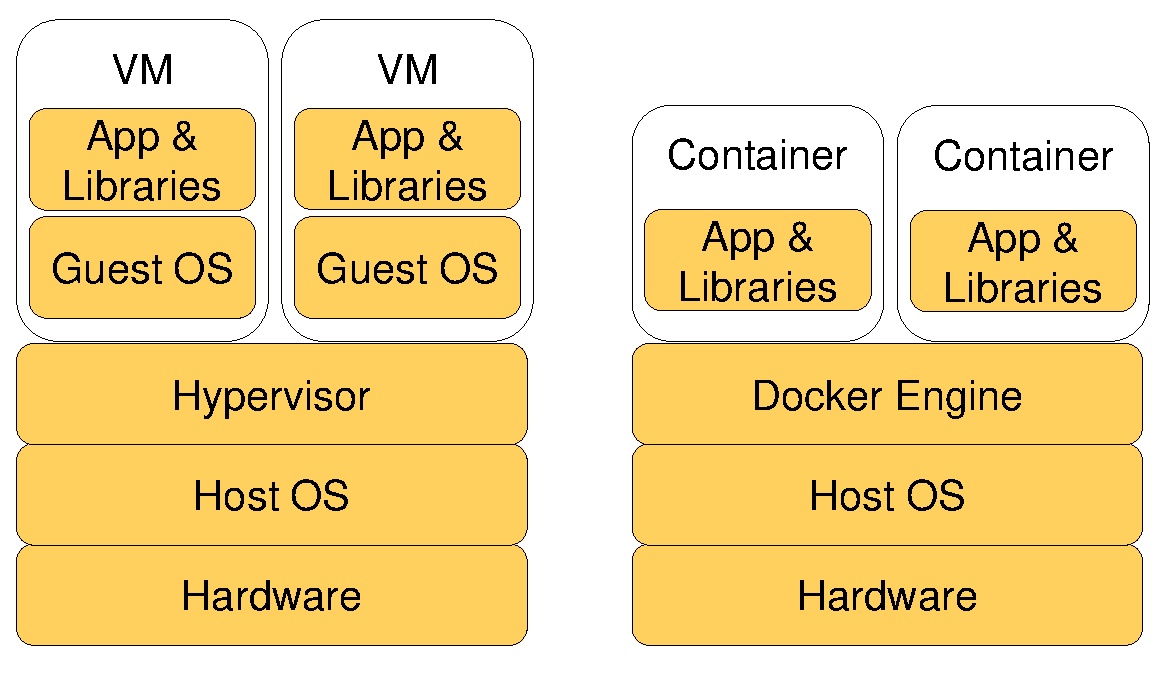
\includegraphics[width=\textwidth]{images/VMxDocker}
		\fonte{Elaborado pelo autor}
	\end{minipage}
\end{figure}

O termo \textit{contêinerização} é a forma popular para se referenciar à virtualização baseada em contêiner, que permite o isolamento de determinados softwares, que são executados dentro do mesmo kernel no sistema operacional Linux, mas que diferentemente do hypervisor, não adiciona uma camada virtualização, na qual precisaria carregar um sistema operacional convidado \cite{Zhang2016}.
Na Tabela~\ref{tab:table1} podemos verificar as diferenças entre as duas tecnologias. Nesta tabela, é importante ressaltar as diferenças de desempenho e tempo de início, os contêineres possuem a vantagem de poder utilizar diretamente os recursos do hospedeiro e não necessitar de tempo de \textit{boot}.

\begin{table}[!ht]
	\caption{Características de VM e contêineres}
	\label{tab:table1}
	\centering
	\resizebox{\textwidth}{!}{%
		\begin{tabular}{|l|l|l|}
			\hline
			\textbf{Parâmetro} &\textbf{Máquinas Virtuais}\ &\textbf{Contêineres}\\
			\hline
			SO Convidado & \begin{tabular}[c]{@{}l@{}}Um hardware virtual é criado para cada\\VM, com um espaço de memória reservado\end{tabular} & \begin{tabular}[c]{@{}l@{}}Todos os convidados compartilham o\\mesmo SO, cada imagem é carregada\\para o espaço de memória do Kernel \end{tabular}\\ \hline
			Comunicação & Feita por dispositivos Ethernet & \begin{tabular}[c]{@{}l@{}} Utilização de mecanismos IPC como sinais,\\sockets, pipes \end{tabular}\\  \hline
			Segurança &\begin{tabular}[c]{@{}l@{}} Depende da implementação do fornecedor\\de hipervisor\end{tabular}& Utilizam mecanismos de controle de acesso\\ \hline
			Desempenho & \begin{tabular}[c]{@{}l@{}}Irá receber uma sobrecarga pelo trabalho\\de tradução de instruções do sistema\\hospedeiro para o convidado\end{tabular}  &\begin{tabular}[c]{@{}l@{}}contêineres fornecem um desempenho\\muito próximo ao nativo em comparação\\ao executado direto no hospedeiro\end{tabular} \\ \hline
			Isolamento &\begin{tabular}[c]{@{}l@{}} Não é possível compartilhar arquivos,\\bibliotecas e execução de programas entre\\as máquinas virtuais  \end{tabular} & \begin{tabular}[c]{@{}l@{}}Subdiretórios podem ser montados e\\compartilhados entre contêineres no mesmo\\hospedeiro \end{tabular} \\ \hline
			Tempo de início & \begin{tabular}[c]{@{}l@{}} Demora o tempo de processo de boot de um \\ sistema operacional \end{tabular} & contêineres não fazem boot de sistema\\ \hline 
			Armazenamento& \begin{tabular}[c]{@{}l@{}}Sistema de arquivos precisa ser\\instalados no convidado além do hospedeiro\end{tabular} & \begin{tabular}[c]{@{}l@{}} O armazenamento em contêineres pode\\ser compartilhado com o hospedeiro \end{tabular} \\ 
			\hline
		\end{tabular}}
		\fonte{\cite{Dua2014}}
\end{table}

\section{Trabalhos Relacionados}
\label{related}
Nesta seção iremos ver um estudo de trabalhos que trazem soluções de elasticidade para aplicações de alto desempenho, bem como estudos comparativos entre a utilização de máquinas virtuais e contêineres, considerados o estado-da-arte na atualidade. Este estudo tem por objetivo confrontar os trabalhos e identificar as lacunas e possíveis melhorias em ambientes elásticos. A seleção de trabalhos relacionados, bem como outras referências, foi realizada através de uma pesquisa em diversas bases de dados de artigos científicos de Ciências Exatas, como o portal da \textit{IEEE Xplore}, \textit{ACM Digital Library} e \textit{Springer Link}, além da bases de dados nacionais, o Portal de Periódicos CAPES/MEC.

Para a realização das pesquisas nessas bases de dados, foram utilizadas buscas com estas principais palavras-chave: \textit{docker virtual machine, container high performance computing, scalablity elasticity, hpc application container, virtualization contêineres, cloud computing elasticity}. O resultado dessas pesquisas foi analisado com o intuito de encontrar trabalhos que explorassem a utilização de contêineres em ambientes de computação em nuvem, bem como as alternativas e implementações de elasticidade em aplicações HPC. 

\subsection{Análise do Estado-da-Arte}
\label{autoelastic}
O AutoElastic, segundo a definição de \citetexto{7090978}, age como um \textit{middleware} permitindo que aplicações HPC iterativas obtenham vantagem do provisionamento dinâmico de recursos de uma infraestrutura de nuvem sem a necessidade de modificações no código fonte. O AutoElastic possui um protótipo executado pelo autor na plataforma de nuvem OpenNebula e obteve resultados de ganho de desempenho de até 59\% na execução de uma aplicação de integração numérica \textit{CPU-Bound}, quando comparada com outras soluções de elasticidade. 

\citetexto{7562612} fazem um estudo comparativo de máquinas virtuais e contêineres, além de propor um modelo de \textit{deploy} de aplicações distribuídas em contêineres Docker. Para verificar o modelo proposto, foram realizados testes utilizando duas aplicações HPC que requerem grande capacidade computacional, Graph500 e Linpack (HPL). Para manter um base de comparação, foram realizados execuções com processamento nativo, sem adição de camada de virtualização. Os testes executados mediam os custos computacionais dos processos, considerando diversas combinações de instâncias de máquinas virtuais e instâncias de contêineres, sem levar em consideração a elasticidade.

\citetexto{Dua2014} apresentam um estudo sobre como provedores de PaaS (\textit{Platform as a Service})estão utilizando contêineres para encapsular aplicações. O estudo indaga a atual adoção de plataformas baseadas em contêineres e explora diversas implementações de contêineres, entre elas: Linux contêineres, Docker, Warden Container, lmctfy e OpenVZ. A análise foi feita baseada em como cada uma das tecnologias lidam com processos, sistema de arquivos e isolamento de namespaces, dando uma atenção especial à características únicas de cada implementação. Por fim, o trabalho busca fazer uma análise dos fatores que afetam a adoção de contêineres e possíveis funcionalidades que estão em falta para uma nova geração de PaaS.

O estudo de \citetexto{Xavier2013} aborda a utilização de tecnologias de virtualização para aplicações de alto desempenho, alegando que tais tecnologias foram tradicionalmente evitadas ao longo dos anos por sua adição de camadas que comprometem desempenho, o que é crucial para tais aplicações. Porém, como o advento de implementações de virtualização baseada em contêineres, o autor indaga que é possível se obter uma sobrecarga muito pequena com a utilização de tecnologias como Linux VServer, OpenVZ e Linux contêineres (LXC), chegando a um desempenho quase nativo. Para comparação, foi utilizado o Xen, um modelo tradicional de virtualização. Os testes utilizaram programas de avaliação de desempenho de supercomputadores fornecidos pela NASA \cite{NASA2016}. O LXC executou os programas de teste com praticamente o mesmo potencial que a própria máquina, enquanto a implementação utilizando máquina virtual (XEN) obteve uma sobrecarga de aproximadamente 4.3\%.

O trabalho de \citetexto{Zhang2016} aborda a sobrecarga que soluções de hipervisor possuem em relação aos dispositivos de I/O virtualizados. O trabalho apresenta SRV-IOV (\textit{Single Root I/O Virtualization }) para permitir o compartilhamento entre conexões de alto desempenho, como InfiniBand, além de introduzir testes utilizando contêineres, buscando atingir um desempenho mais próximo do nativo. Nos testes, utilizando aplicações de \textit{benchmark} com MPI, as avaliações identificaram que VM com passagem PCI é mais eficiente que VM com SR-IOV habilitado, entretanto, contêineres possuem mais eficiência ao compartilhar recursos de I/O. Em comparação ao desempenho nativo, os testes identificaram uma sobrecarga para contêineres de no máximo 9\% para aplicações HPC.

\citetexto{Adufu2015} conduziram testes para demonstrar que, durante a execução de aplicações científicas em ambientes HPC, o tempo médio de processamento em um sistema com virtualização baseada em contêineres é menor do que o tempo em um sistema baseado em \textit{hypervisor}, isto devido ao tempo de \textit{start-up}. Para gerar os resultados de comparação, foi utilizado a ferramenta \textit{autodock3}, um programa de simulação de modelagem molecular. Para gerenciar os contêineres, a ferramenta Docker foi utilizada, mostrando um gerenciamento de recursos mais eficiente, até mesmo no cenário em que foi alocado mais memória do que realmente disponível fisicamente para as instâncias em execução. 

\citetexto{Kominos2017} fazem uma análise sobre as opções de provisionamento na plataforma OpenStack, que são: máquinas virtuais, contêineres e \textit{bare-metal} (instalação do zero nas máquinas). As alternativas são comparadas em relação à CPU, networking, operações de I/O e acesso à RAM, além de medição de tempo de \textit{boot}. Contêineres Docker container apresentaram o tempo de início mais rápido, e obteve um desempenho muito próximo do \textit{bare-metal} nos outros quesitos, este que por sua vez, teve os melhores resultados. Em geral, VMs obtiveram os piores resultados, principalmente em relação ao desempenho de múltiplas vCPUs.

O artigo de \citetexto{Molto2017} descreve um \textit{workflow} para permitir a execução de uma aplicação tanto em ambientes virtualizados, como em ambientes baseados em contêineres, o que foi chamado de Infraestrutura Híbrida de Computação Distribuída (IHCD), utilizando ferramentas open-source do projeto INDIGO-DataCloud. O principal problema abordado é a falta de interoperabilidade de uma imagem entre hipervisores (VMs) e contêineres. O resultado é uma ferramenta que permite a criação de um \textit{template} com as especificações necessárias da aplicação e a plataforma OpenNebula cria a imagem e a disponibiliza conforme solicitado (Docker ou VM). O tempo total deste processo para uma aplicação de teste é de 20:48 (minutos:segundos) para VM e 7:25 para Docker.

Para finalizar, \citetexto{Zheng2017} avaliam as diferenças fundamentais entre Docker e máquinas virtuais, contrariando os outros trabalhos relacionados, porquê apresenta situações onde máquinas virtuais podem apresentar um desempenho melhor que contêineres Docker. Nos benchmarks executados, o Docker atingiu um gargalo de velocidade em operações de disco de byte-a-byte, enquanto os testes com VMs atingiram resultados parecidos com o desempenho nativo para resolver o problema N-Queens. Mesmo assim, o trabalho ressalva que as diferenças de \textit{overhead} de desempenho entre os tipos de virtualização ocorrem não somente no modo implementado, como também depende da aplicação em execução. 

\subsection{Discussão e Lacunas}
\label{comparacao}
Até esta seção, foram mostrados os estudos existentes para implementações de soluções de desenvolvimento de aplicações HPC, que utilizam os dois conceitos de virtualização, baseado em contêineres e em \textit{hypervisor}. Na tabela \ref{tab:table2} é feito um resumo do resultado destes estudos, elencando as principais características dos trabalhos conduzidos. Podemos notar que, apesar do trabalho de Facco \citetexto{Facco2016} apresentar um modelo elástico para aplicações HPC, não existem outros estudos que mostrem o comportamento de contêineres sob estas condições. Os demais trabalhos fazem uma análise do desempenho de contêineres, porém sem instanciação dinâmica de contêineres pelo gerenciador, o que daria o aspecto de um sistema elástico.

\begin{table}[]
\centering
\caption{Comparação de trabalhos relacionados}
\label{tab:table2}
\resizebox{\textwidth}{!}{%
\begin{tabular}{|l|l|l|l|l|l|l|}
\hline
\textbf{Trabalho} & \textbf{Tecnologia}  & \textbf{Elasticidade} & \begin{tabular}[c]{@{}l@{}}\textbf{Base de}\\\textbf{Comparação} \end{tabular}     & \textbf{Métricas}                                                                   & \textbf{Plataforma}  & \textbf{Testes}                                                              \\ \hline
\cite{Facco2016}       & VM                   & Sim                   & Ubuntu 10.04 &\begin{tabular}[c]{@{}l@{}} desempenho, custo e\\ energia\end{tabular}                                                          & OpenNebula           & cálculo de integrais                                                         \\ \hline
\cite{7562612}                 & Docker               & Não                   & CentOS 7 3.10         & \begin{tabular}[c]{@{}l@{}} Performance por \\instancias  \end{tabular}                                                        & OpenStack            & \begin{tabular}[c]{@{}l@{}} MPI com Graph500,\\ Linpack\end{tabular}                                                   \\ \hline
\cite{Xavier2013}                 & \begin{tabular}[c]{@{}l@{}} LXC, OpenVZ,\\ VServer \end{tabular} & Não                   & Ubuntu 10.04               & \begin{tabular}[c]{@{}l@{}}diversos tipos de \\ recursos em único nó\end{tabular} & Não & \begin{tabular}[c]{@{}l@{}}Linpack, STREAM, \\ IOZone, NetPIPE\end{tabular} \\ \hline
\cite{Zhang2016}                 & Docker               & Não                   & CentOS Linux                    & \begin{tabular}[c]{@{}l@{}}desempenho \\ de comunicação\end{tabular}    & OpenStack            & \begin{tabular}[c]{@{}l@{}}MPI com Graph500,\\ NAS, LAMMPS\end{tabular}     \\ \hline
\cite{Adufu2015}                 & Docker               & Não                   & Ubuntu 14.04& \begin{tabular}[c]{@{}l@{}}Desempenho de RAM\end{tabular}                & OpenStack            & \textit{autodock3}                                                                    \\ \hline
\cite{Kominos2017} & Docker& Não & Ubuntu 14.04&\begin{tabular}[c]{@{}l@{}} Desempenho de CPU,\\ rede, RAM e disco\end{tabular}& OpenStack &\begin{tabular}[c]{@{}l@{}} ParallelPXZ,\\ Netperf, SysBench \end{tabular}\\ \hline
\cite{Molto2017} & Docker & Não & Ubuntu 14.04 & Provisionamento& OpenNebula & Tempo médio \\ \hline
\cite{Zheng2017} & Docker & Não & Ubuntu 15.10 &\begin{tabular}[c]{@{}l@{}} Desempenho de CPU,\\disco e RAM\end{tabular} & Não &\begin{tabular}[c]{@{}l@{}} Iperf, STREAM,\\HardInfo, Bonnie++\end{tabular}\\ \hline
\end{tabular}}
\fonte{Elaborado pelo autor}
\end{table}

Os estudos mostrados na tabela \ref{tab:table2} que abordaram a utilização da tecnologia de contêineres, exibem resultados mais favoráveis à estas implementações em comparação ao método tradicionais de virtualização, abordando diversos aspectos inerentes à virtualização de recursos, como operações de I/O, desempenho de memória RAM e consumo de energia. Todos estes são aspectos fundamentais para uma solução de ambiente HPC eficiente. Embora os trabalhos mostrem resultados aplicando programas de \textit{benchmark} para medir o desempenho da infraestrutura, não foi encontrado um estudo que verificasse o desempenho elástico de contêineres para um modelo de provisionamento de recursos de forma dinâmica, como o AutoElastic mostra, utilizando máquinas virtuais.

Sendo assim, os trabalhos analisados deixaram uma lacuna em relação a esta questão, por não apresentarem uma solução dinâmica e elástica, que utilize uma tecnologia mais eficiente para processamento do que máquinas virtuais para alocação de recursos. É possível, então, aproveitar essa lacuna e fazer uma validação da elasticidade de aplicações HPC com contêineres, através de modificações no modelo AutoElastic para suportar essa tecnologia em suas operações.

%=======================================================================
% Modelo
%=======================================================================
\section{Benchmark DoCB}
\label{model}

Neste capítulo apresentaremos o modelo do Docker Containers Benchmark (DoCB), uma análise de viabilidade de elasticidade em nuvem para contêineres, em comparação ao modelo tradicional, que utiliza máquinas virtuais. e debateremos em termos gerais as questões de projeto na seção \ref{questao}. Na próxima seção \ref{arquitetura}, abordaremos sua arquitetura. 

\subsection{Questões de projeto}
\label{questao}

Para obter a elasticidade em nuvem, utilizaremos a ferramenta AutoElastic. Nesse caso, iremos adicionar ao componente de criação de recursos a possibilidade de instanciar contêineres além máquinas virtuais, ficando transparente ao usuário essa opção, minimizando a configuração necessária para utilização das opções de virtualização. A elasticidade se dará no momento em que a aplicação decidir adicionar recursos para otimizar a execução das aplicações, utilizando os critérios definidos. Como as imagens de contêineres possuem um tamanho significativamente menor que o de uma máquina virtual, o gerenciador poderá lançar \textit{n} instâncias de contêineres para um mesmo host, obtendo vantagens ao executar aplicações paralelas. 

O gerenciador AutoElastic foi escolhido por permitir virtualização de acordo com a utilização dos recursos computacionais já alocados. A elasticidade aplicada pelo gerenciador será horizontal, ou seja, a elasticidade é aplicada ao alocar e desalocar recursos virtualizados, e não na configuração de hardware. A métrica utilizada pelo gerenciador será a média de CPU dos contêineres alocados, pois o AutoElastic utiliza a média de CPU das máquinas virtuais para tomada de decisão.

\subsection{Arquitetura}
\label{arquitetura}
Este trabalho parte da implementação do modelo AutoElastic para propor uma modificação em sua arquitetura, acrescentando a possibilidade de utilizar contêineres ao invés de máquinas virtuais. O AutoElastic é um \textit{middleware} que permite que o usuário possa obter elasticidade para suas aplicações, sem depender de alterações no código-fonte. Operando no nível de PaaS, o modelo permite que aplicações iterativas obtenham elasticidade através de operações de alocação e consolidação de instâncias de máquinas virtuais em nós físicos. O \textit{framework} atual é composto por um Gerenciador, um componente independente da infraestrutura, não interferindo no resultado da execução e podendo gerenciar os recursos remotamente, através do acesso de um computador \textit{frontend} do \textit{cluster} de computadores.

A figura \ref{fig:arquitetura} mostra como é a arquitetura do modelo proposto. Cada nó possui um gerenciador de container, o Docker. O número de contêineres pode partir de 1 contêiner por nó, a partir do contêiner do processo mestre da aplicação, até vários contêineres por nó, definido pelo usuário do gerenciador \cite{6307065}.

\begin{figure}
	\caption{Arquitetura do Modelo. Aqui, \textit{n} representa o número de nós disponíveis, e \textit{m} o número de Docker contêineres.}
	\label{fig:arquitetura}
	\centering%
	\vspace{-0.5\baselineskip}
	\begin{minipage}{0.8\textwidth}
		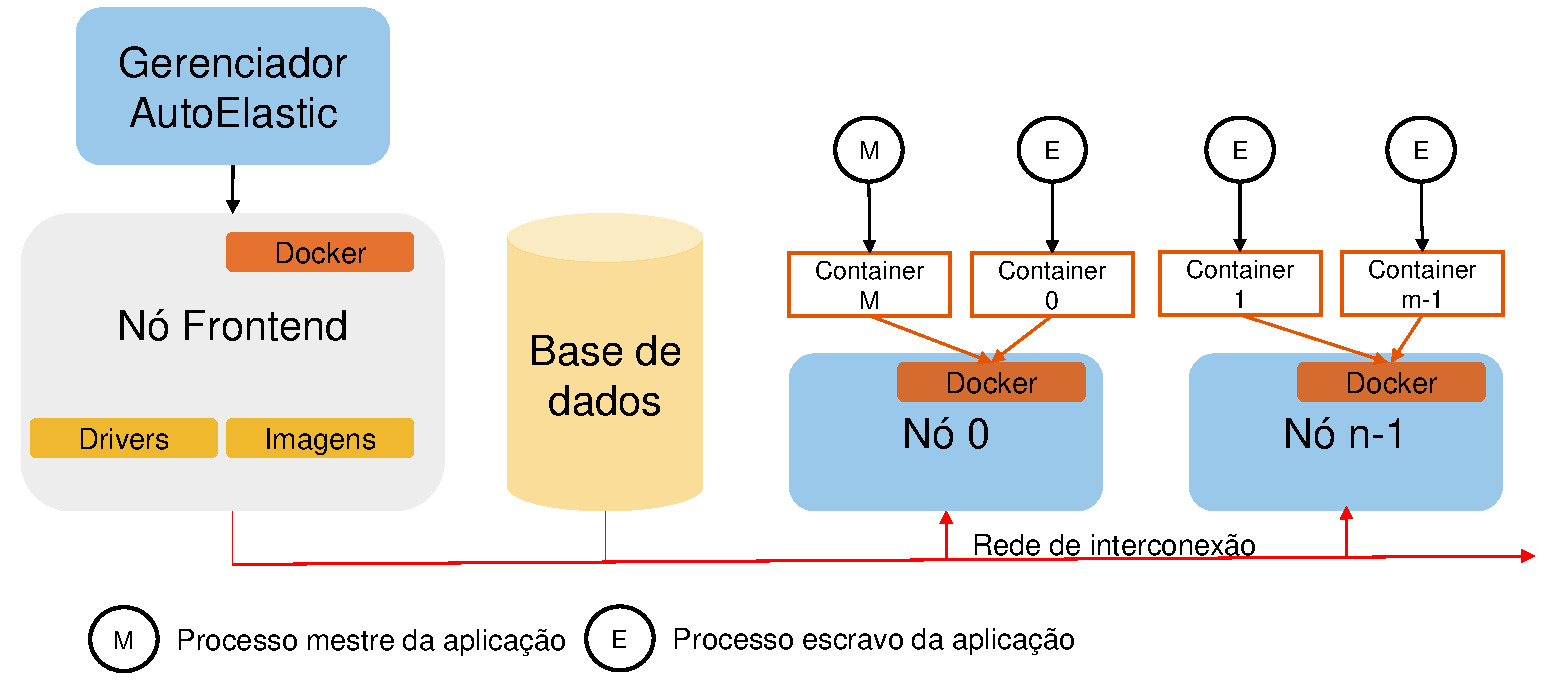
\includegraphics[width=\textwidth]{images/arquitetura}
		\fonte{Elaborado pelo autor}
	\end{minipage}
\end{figure}

O gerenciador analisa periodicamente as instâncias de contêineres que estão ativas, e verifica se é necessário um adição ou remoção de recursos, dependendo da configuração de \textit{threshold}. No modelo proposto, o usuário pode definir o número minimo e máximo de contêineres por nó e quantos poderão operar na execução da aplicação. Ainda, a arquitetura garante que a aplicação em execução não tem o seu desempenho afetado pela adição ou remoção de recursos, pois o gerenciador atua de forma isolada do \textit{cluster} de computadores. 

A base dados mostrada na figura \ref{fig:arquitetura} é utilizada para armazenar as imagens utilizadas pelo nó \textit{frontend}, além de permitir um espaço de comunicação entre o gerenciador e as instâncias de contêineres em execução, sendo este espaço acessável apenas pelos computadores do \textit{cluster}. A utilização de uma área compartilhada, para comunicação entre computadores virtualizados é uma prática comum, quando se falando de nuvens privadas. No contexto de Docker, a base de dados é um banco local \textit{Docker Repository} e a área de dados comum é montada pelos contêineres utilizando a ferramenta de \textit{volumes}, que monta um diretório compartilhado.

\subsection{Elasticidade}
As aplicações de HPC normalmente lidam com computação intensiva, por esse motivo, iremos nos concentrar apenas na métrica de CPU para tomada de decisão. O Gerenciador captura periodicamente os valores de carga de CPU dos objetos virtualizados (máquina virtual ou contêiner) que estão executando os processos. É feita uma média desses valores e estes são armazenados juntamente com coletas operações anteriores para realizar o cálculo de carga geral. O valor resultante do cálculo é avaliado conforme regras definidas de \textit{threshold} superior e inferior, que são definidos por valores de 0\% a 100\% respectivamente. 

O AutoElastic possui em sua implementação algumas opções de algoritmo de avaliação, entre elas o algoritmo que opera segundo o conceito \textit{Aging}. Segundo \citetexto{Tanenbaum03}, a técnica utiliza uma suavização exponencial simples, aplicando maior peso para a última coleta para definir a carga. O algoritmo permite suavizar picos de carga (superior e inferior), evitando operações de elasticidade desnecessárias, causadas por falso-positivos em termos de atingir um \textit{threshold}. Podemos ver, na Figura~\ref{fig:aging}, um caso simples onde as operações de elasticidade ocorreriam se fosse considerado apenas a carga real medida, porém, com a técnica de \textit{Aging}, evitamos estas operações de elasticidade. Assim, foi escolhido esse algoritmo para evitar ruídos nas leituras que possam prejudicar a execução eficiente da aplicação. Os \textit{thresolds} superior e inferior são fixos, sendo esses informados previamente antes do iniciar o monitoramento.

\begin{figure}
	\caption{Utilização da técnica de \textit{Aging} para alocar e desalocar recursos de de forma suavizada}
	\label{fig:aging}
	\centering%
	\vspace{-0.5\baselineskip}
	\begin{minipage}{0.75\textwidth}
		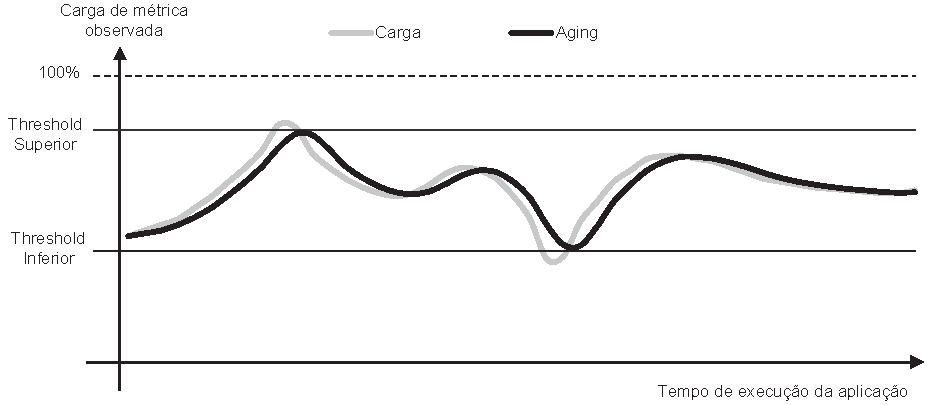
\includegraphics[width=\textwidth]{images/aging}
		\fonte{\cite{Facco2016}}
	\end{minipage}
\end{figure}

\subsection{Estratégia de Execução}

Fluxograma

Falar de Rígido e Flexível.

\section{Metodologia de Avaliação}
Apresentar a seção

\subsection{Implementação}
\label{prototype}

Para a execução dos experimentos em nuvem, utilizaremos o protótipo desenvolvido por Facco \citetexto{Facco2016}, que consiste de uma aplicação em Java para gerenciamento de elasticidade, o AutoElastic. O modelo será estendido, passando a considerar a utilização de contêineres. O protótipo atual consiste de uma ferramenta que gerencia uma nuvem OpenNebula, sendo o controle do ambiente realizado através de uma API em Java que o \textit{middleware} OpenNebula oferece, como por exemplo, a criação de máquinas virtuais dentro do \textit{cluster}. 

Escolhemos o Docker como ferramenta de manipulação de contêineres, justamente pela sua facilidade de gerenciar contêineres e estabelecer um padrão de utilização muito aceito pelo mercado. A plataforma OpenNebula fornece extensões para permitir a utilização do Docker ao invés de Máquinas Virtuais, conforme a sua documentação por Laguna \citetexto{onedock2015}:

\begin{quote}
ONEDock é um conjunto de extensões para o OpenNebula para utilização de Docker contêineres como entidades de primeira classe, assim como se fossem Máquinas Virtuais (VM) leves. Para tal, Docker é configurado para atual como um \textit{hypervisor}, comportando-se então, como o KVM ou outro \textit{hypervisor} fazem no contexto de OpenNebula.
\end{quote} 

Este conjunto de ferramentas é open-source, o que possibilitou a codificação de características não suportadas pela distribuição atual da ferramenta, como veremos logo adiante na seção \ref{avaliacao}.

\subsubsection{Acesso à rede}
O OpenNebula permite que seja definida uma interface de rede no momento de deploy de uma máquina virtual, porém o Docker possui uma configuração própria de interface de rede para o computador no qual está sendo executado, que é visível para todos os contêineres em execução na mesma máquina, porém não acessível de fora deste computador. Cada computador possui um processo Docker que gerencia os contêineres, a entrega de uma imagem do frontend para os nós é feita através de entrega da imagem no diretório compartilhado e execução remota de comandos Docker, como mostrado na figura \ref{fig:provision-use-case}.

\begin{figure}
	\caption{Formato de provisionamento de container Docker}
	\label{fig:provision-use-case}
	\centering%
	\begin{minipage}{0.8\textwidth}
		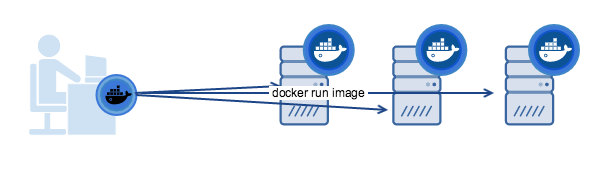
\includegraphics[scale=0.6]{provision-use-case}
		\fonte{\cite{whitepaperDocker2016}}
	\end{minipage}
\end{figure}


Os contêineres lançados possuem acesso somente à esta rede isolada. Portanto, para que todos os contêineres gerenciados pelo OpenNebula possam se comunicar, a tecnologia permite que determinadas portas do container sejam redirecionadas para portas do host, a figura \ref{fig:network_access} mostra como esta comunicação é feita. Esta abordagem foi aplicada aos contêineres para permitir a troca de mensagens entre os contêineres distribuídos em diferentes máquinas da Nuvem.
\begin{figure}
	\caption{Redirecionamento de portas para contêineres}
	\label{fig:network_access}
	\centering%
	\begin{minipage}{0.8\textwidth}
		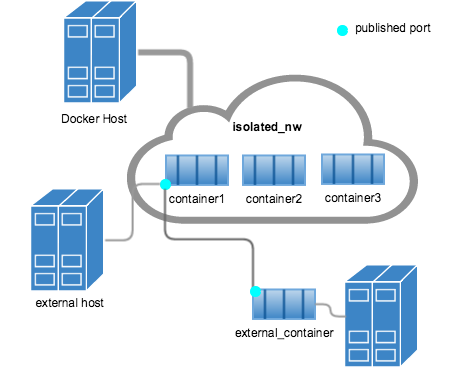
\includegraphics[width=\textwidth]{network_access}
		\fonte{\cite{whitepaperDocker2016}}
	\end{minipage}
\end{figure}


\subsection{Cenários}
\label{cenarios}

Para a execução dos cenários de teste, estaremos utilizando a aplicação desenvolvida por \citetexto{Facco2016}, o programa consiste de um código para rodar cálculos de integrais em uma rede, seguindo o modo master-slave, sob diferentes tipos de carga, no nosso caso, utilizaremos a carga ascendente e descendente. O objetivo da aplicação é irrelevante, pois ela será utilizada apenas para fazer o benchmarking dos cenários de elasticidade. A aplicação realizará cálculos numéricos e distribuirá porções de trabalho para cada nó, interligados por MPI. A aplicação fica ciente de novos nós disponíveis a partir de um sistema de comunicação através de arquivos de texto, disponibilizados pela aplicação AutoElastic durante as operações de provisionamento de recursos.


%The
%prototype was used to run a numerical integration application
%over a private cloud under different situations of load
%(Ascending, Descending, Wave and Constant). The goal is
%to show the AutoElastic actions considering the load
%changes and the impact of both the loads and the asynchronism
%on the applications performance.

%The application used in the tests computes the numerical
%integration of a function f(x) in a closed interval ½a; b. It was
%implemented using the Composite Trapezoidal rule from a
%Newton-Cotes postulation [46]. The Newton-Cotes formula
%can be useful if the value of the integrand is given at equally
%spaced points. Considering the partition of the interval ½a; b
%into s equally spaced subintervals, each one with length h

Considerando a infraestrutura já mencionada, cada nó foi exclusivamente dedicado para execução do benchmarking, sendo a aplicação do AutoElastic executava em um computador fora da Nuvem, utilizando a API do OpenNebula para controle dos recursos. O SLA foi configurado diferentemente para cada tipo de cenário, porém o número de hosts físicos foi fixado em 4, além de 1 host para o front-end. 

\subsubsection{Execução com VMs}

O DoCPB (Docker contêineres Parallel Benchmarking) contará com uma execução do AutoElastic configurado para instanciar máquinas virtuais, que servirá como base de comparação, sendo que este é considerado o estado da arte do modelo. Para tal, dois templates de imagens foram configurados com o sistema operacional Ubuntu 10.10, sendo o master provido com 1 unidade de CPU e 1GB de RAM, além do template slave com 1 unidade de CPU e 2GB de RAM, desta forma, cada vez que for solicitado por um recurso adicional de computação, uma unidade slave é carregada para um dos nós de computação, ocupando 1 dos cores de CPU e metade da memória RAM disponível.

\subsubsection{Execução com contêineres}

A execução da aplicação paralela com configuração de 2 VMs por hosts (1 para cada core) é considerada a mais otimizada, segundo \citetexto{Facco2016}. Porém, não sabemos se a mesma regra se aplica ao cenário de contêineres, por serem processos mais leves que uma máquina virtual, é possível que um número maior de contêineres por nó tenha um desempenho melhor. Tendo em vista isto, criamos os cenários de acordo com a tabela \ref{tab:table3}.

\begin{table}[]
\centering
\caption{Cenários de contêineres}
\label{tab:table3}
\begin{tabular}{|l|l|l|l|l|}
\hline
\textbf{Cenário} & \textbf{Slaves Inicial} & \textbf{CPU alocada} & \textbf{RAM alocada (GB)} & \textbf{contêineres por operação} \\ \hline
1                & 1                       & 2                    & 4096                      & 1                                \\ \hline
2                & 2                       & 1                    & 2048                      & 2                                \\ \hline
3                & 2                       & 0.5                  & 1024                      & 4                                \\ \hline
4                & 2                       & 0.25                 & 512                       & 8                                \\ \hline
\end{tabular}
\end{table}

\begin{figure}
	\caption{Redirecionamento de portas para contêineres}
	\label{fig:deploy}
	\centering%
	\begin{minipage}{0.8\textwidth}
		\vspace{-0.5\baselineskip}
		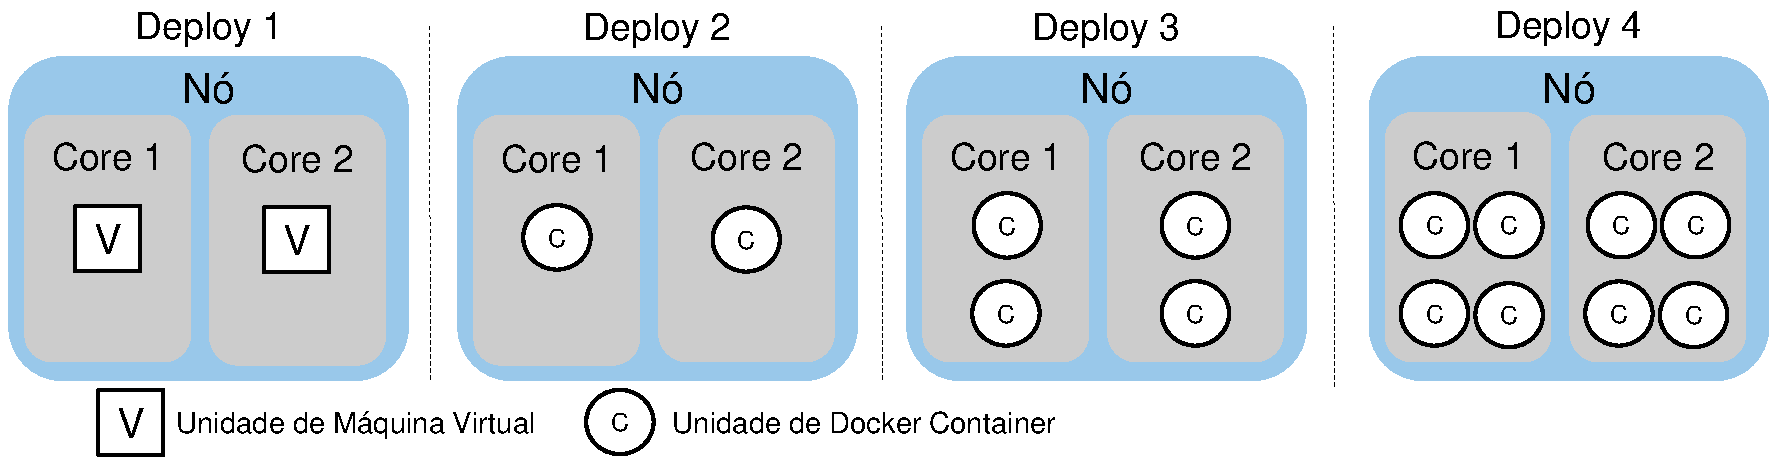
\includegraphics[width=\textwidth]{images/deploy}
		\fonte{\cite{whitepaperDocker2016}}
	\end{minipage}
\end{figure}
No cenário 1 da tabela, alocamos toda a capacidade de processamento (CPU) e de memória disponível do host, sendo que cada operação de alocação de recursos irá adicionar 1 container em um outro host, ocupando toda a capacidade deste para execução deste container também. No cenário 2, temos uma configuração considerada equivalente ao definido para o cenário de máquinas virtuais, ou seja, 2 contêineres por operação, sendo cada um com 1 core da CPU e 2GB de memória RAM. Temos outros dois cenários estabelecidos para avaliação, o cenário 3 com configuração para ocupar cada nó de processamento com 4 contêineres e o cenário 4 com configuração para 8 contêineres por nó, sendo estes também configurados para ocupar toda a capacidade do nó.





There are some technical decisions that are imposed in
the implementation of the AutoElastic prototype: (i) utilization
of network file system to implement the AutoElastic
module responsible for providing a private area for data
sharing inside the cloud; (ii) AutoElastic employs periodic
monitoring, which is associated with a period of 30 s (Open-
Nebula lower bound index); and (iii) Contemplating related
work, 80 and 40 percent were used for maximum and minimum
thresholds. Looking at decision (i), the manager uses
the binary SCP from the SSH package to obtain or place files
from/to the cloud front-end. These files are in a shared
folder that is enabled with NFS and represents elasticity
actions and process data. We follow this implementation
because the AutoElastic Manager cannot access the NFS
directly, unless it is placed inside the cloud.

\subsubsection{Infraestrutura}

Como infraestrutura de nuvem, utilizaremos o ambiente disponibilizado pela Universidade do Vale do Rio dos Sinos, localizado no laboratório C01 413 do Programa de Pós-Graduação em Computação Aplicada (PIPCA). O laboratório conta com 18 computadores, interconectados através de uma rede 100Mbps, sendo a configuração de cada um deles uma memória de 4 GB, além de processadores de dois núcleos de 2.9 GHz. Porém, para fins de teste de cenários específicos deste trabalho, 5 máquinas do laboratório foram configuradas para serem utilizadas. A plataforma de nuvem OpenNebula será instalada nesta rede de computadores para a execução do protótipo, sendo que uma das máquinas será utilizada como nó \textit{Front-End}. 
A versão 1.1 do ONEDock tem suporte mínimo para a distribuição 4.14 do OpenNebula, portanto esta também teve que ser instalado. Além disto,a versão 1.9 do Docker foi escolhida por ser a versão no qual o ONEDock 1.1 foi testado. 

\subsection{Métricas e Parâmetros}
Falar dos thresholds escolhidos

De acordo com <cite alguem>, para mantermos o 
calcular número de CPUs utilizadas??


Therefore, considering the values of the cost in
Table 4, the objective is to preserve the truth of
Inequality (7):
Fig. 6. (a) Template of the input file for the tests; (b), (c), (d) and (e) are Cost App Time Resource



As técnicas de análise de \textit{Speedup} Elástico e Eficiência Elástica serão utilizadas para medir o desempenho de elasticidade de de nuvem em aplicações HPC \cite{Facco2016}. O \textit{Speedup} Elástico será utilizado para identificar a elasticidade do modelo em duas situações, uma com modelo configurado para um processo único executando a aplicação, e no outro será analisado o desempenho da execução em paralelo. A técnica de análise de Eficiência Elástica será utilizada, pois é pertinente identificar o quão eficiente é o modelo em questão de utilização dos recursos disponíveis, considerando sempre a elasticidade horizontal, ou seja, adicionando ou removendo recursos através de provisionamento de novas instâncias. 

A partir da utilização de tais técnicas de avaliação, pode-se considerar vários cenários de implementação da nuvem, ou seja, as combinações serão exploradas independente de quantos núcleos de processamento estão disponível para cada nó computacional, isto com o objetivo de identificar as situações em que os modelos terão comportamentos discrepantes. Dessa forma, será feita também uma análise comparando o tempo de provisionamento dos recursos, levando em consideração todos os momentos envolvidos, que são: a busca da imagem no nó principal, o tempo de transferência desta imagem para o nó de execução, o tempo de criação da instância a partir da imagem e o tempo de inicialização da instância para rodar a aplicação. Estes passos são considerados tanto para máquinas virtuais quanto contêineres. 

Falar de Energia e Custo




\section{Resultados}
\label{avaliacao}

Esta seção apresenta detalhes sobre o benchmarking DoCPB executado e também irá cobrir os resultados, conforme comentado na seção `introdução'. 



\begin{figure}%
\centering
\subfloat[2 VM's por host]{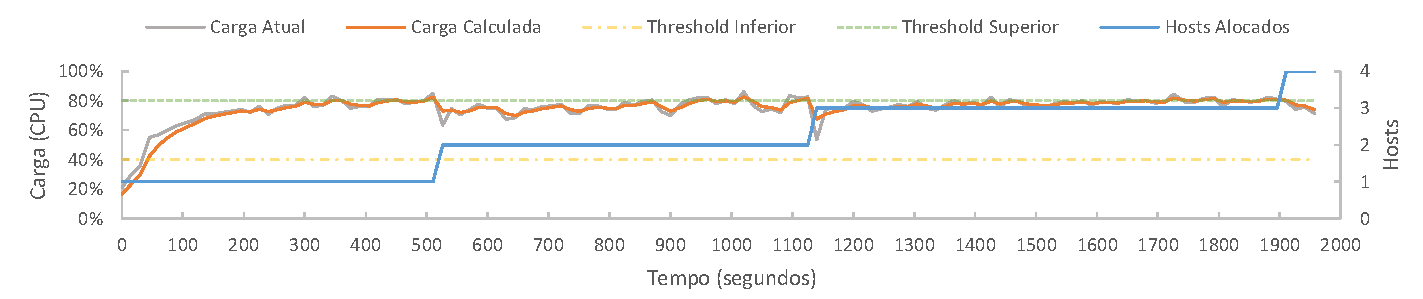
\includegraphics[width= 15cm]{charts/vmelastic.pdf}}\\
\vspace{-0.5\baselineskip}
\subfloat[2 contêineres por host (CPU Rígido)]{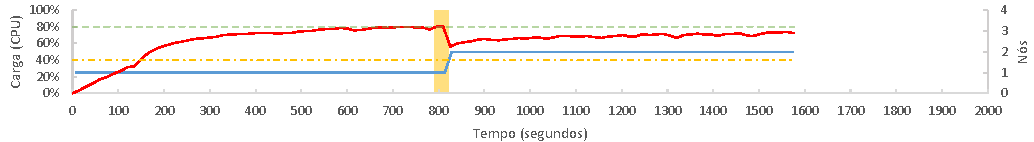
\includegraphics[width= 15cm]{charts/asc2contFixo.pdf}}\\
\vspace{-0.5\baselineskip}
\subfloat[2 contêineres por host (CPU Flexível)]{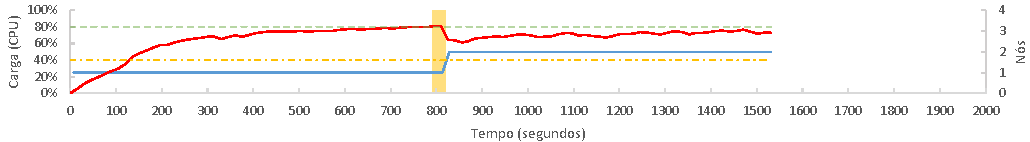
\includegraphics[width= 15cm]{charts/asc2contFlex.pdf}}\\
\vspace{-0.5\baselineskip}
\subfloat[4 contêineres por host (CPU Rígido)]{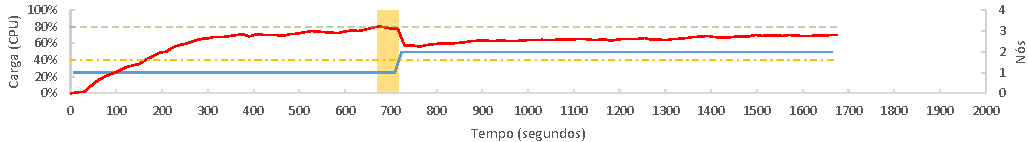
\includegraphics[width= 15cm]{charts/asc4contFixo2.pdf}}\\
\vspace{-0.5\baselineskip}
\subfloat[4 contêineres por host (CPU Flexível)]{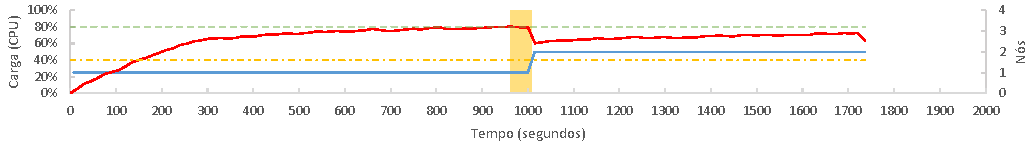
\includegraphics[width= 15cm]{charts/asc4contFlex.pdf}}\\
\vspace{-0.5\baselineskip}
\subfloat[8 contêineres por host (CPU Rígido)]{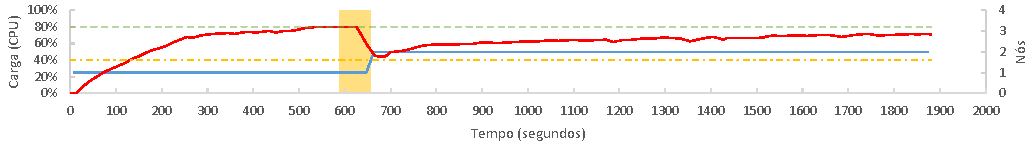
\includegraphics[width= 15cm]{charts/asc8contFixo.pdf}}\\
\vspace{-0.5\baselineskip}
\subfloat[8 contêineres por host (CPU Flexível)]{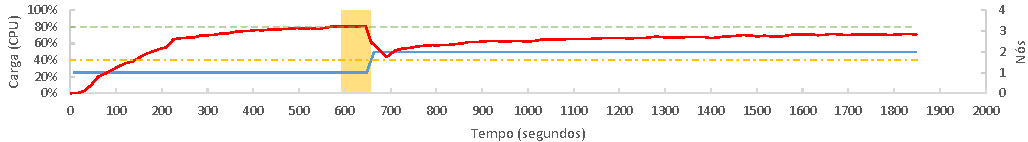
\includegraphics[width= 15cm]{charts/asc8contFlex.pdf}}\\
\caption{Tendência de tempo de execução de aplicação ascendente variando o número de instâncias por host alocado}
\label{fig:trend_asc}
\end{figure}


\begin{figure}%
\centering
\subfloat[2 VM's por host]{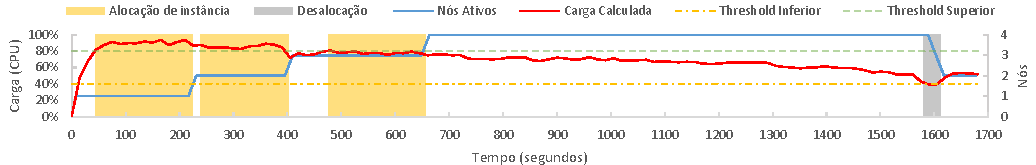
\includegraphics[width= 15cm]{charts/desVMFixo.pdf}}\\
\vspace{-0.5\baselineskip}
\subfloat[2 contêineres por host (CPU Rígido)]{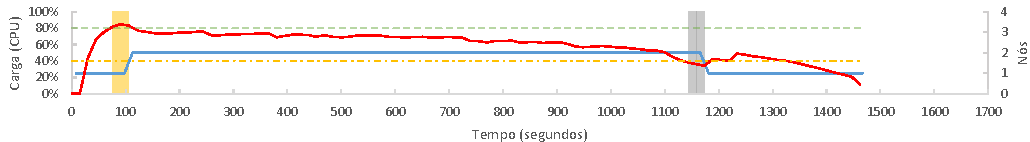
\includegraphics[width= 15cm]{charts/des2contFixo.pdf}}\\
\vspace{-0.5\baselineskip}
\subfloat[2 contêineres por host (CPU Flexível)]{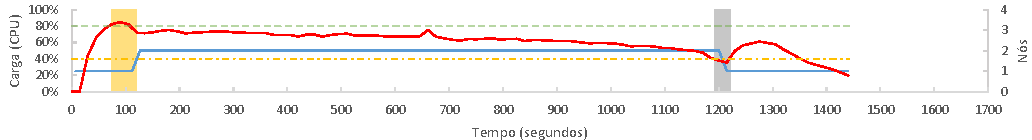
\includegraphics[width= 15cm]{charts/des2contFlex.pdf}}\\
\vspace{-0.5\baselineskip}
\subfloat[4 contêineres por host (CPU Rígido)]{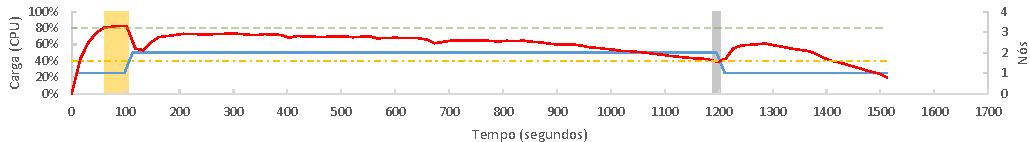
\includegraphics[width= 15cm]{charts/des4contFixo.pdf}}\\
\vspace{-0.5\baselineskip}
\subfloat[4 contêineres por host (CPU Flexível)]{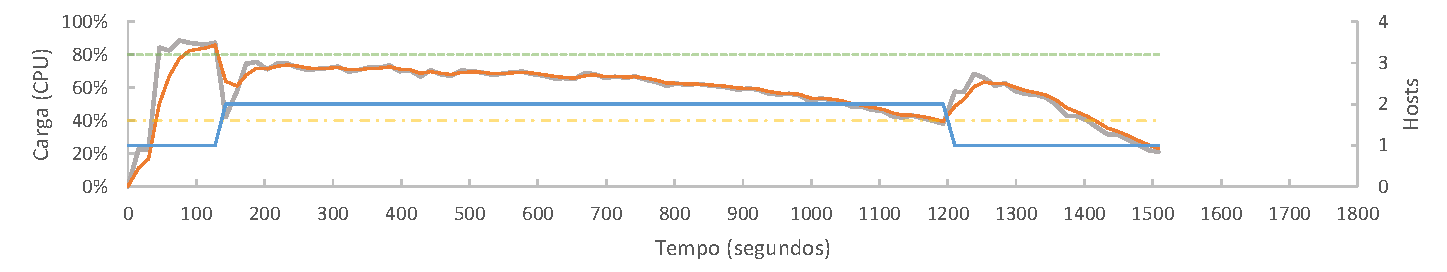
\includegraphics[width= 15cm]{charts/des4contFlex.pdf}}\\
\vspace{-0.5\baselineskip}
\subfloat[8 contêineres por host (CPU Rígido)]{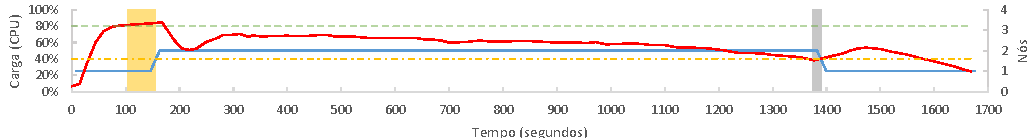
\includegraphics[width= 15cm]{charts/des8contFixo.pdf}}\\
\vspace{-0.5\baselineskip}
\subfloat[8 contêineres por host (CPU Flexível)]{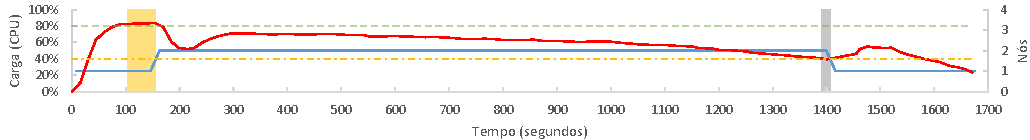
\includegraphics[width= 15cm]{charts/des8contFlex.pdf}}\\
\caption{Tendência de tempo de execução de aplicação descendente variando o número de instâncias por host alocado e atingindo threshold superior e inferior}
\label{fig:trend_des}
\end{figure}

\begin{figure}%
\centering
\subfloat{
\includegraphics{charts/cropped_legendas.pdf}}\\
\setcounter{subfigure}{0}%
\subfloat[][]{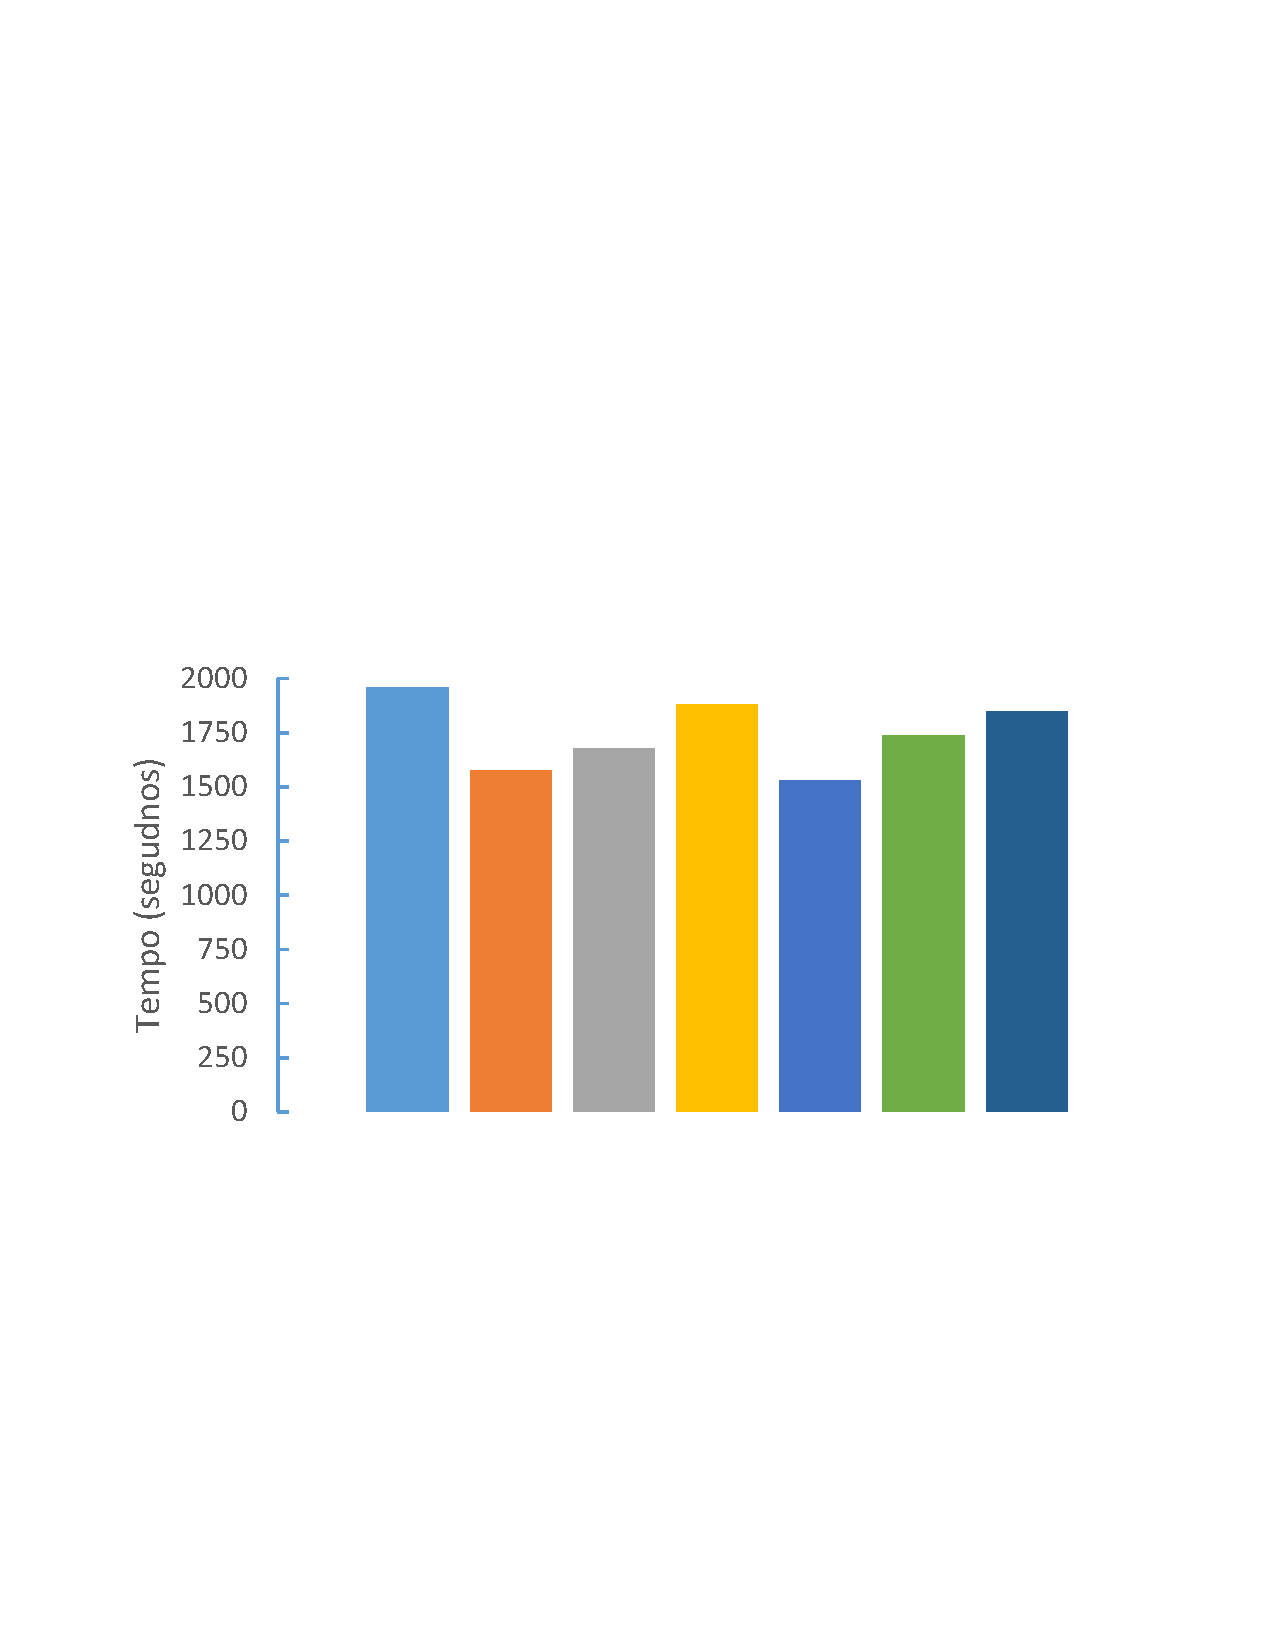
\includegraphics[width= 5cm]{charts/tempo_asc.pdf}}\
%\qquad
\subfloat[][]{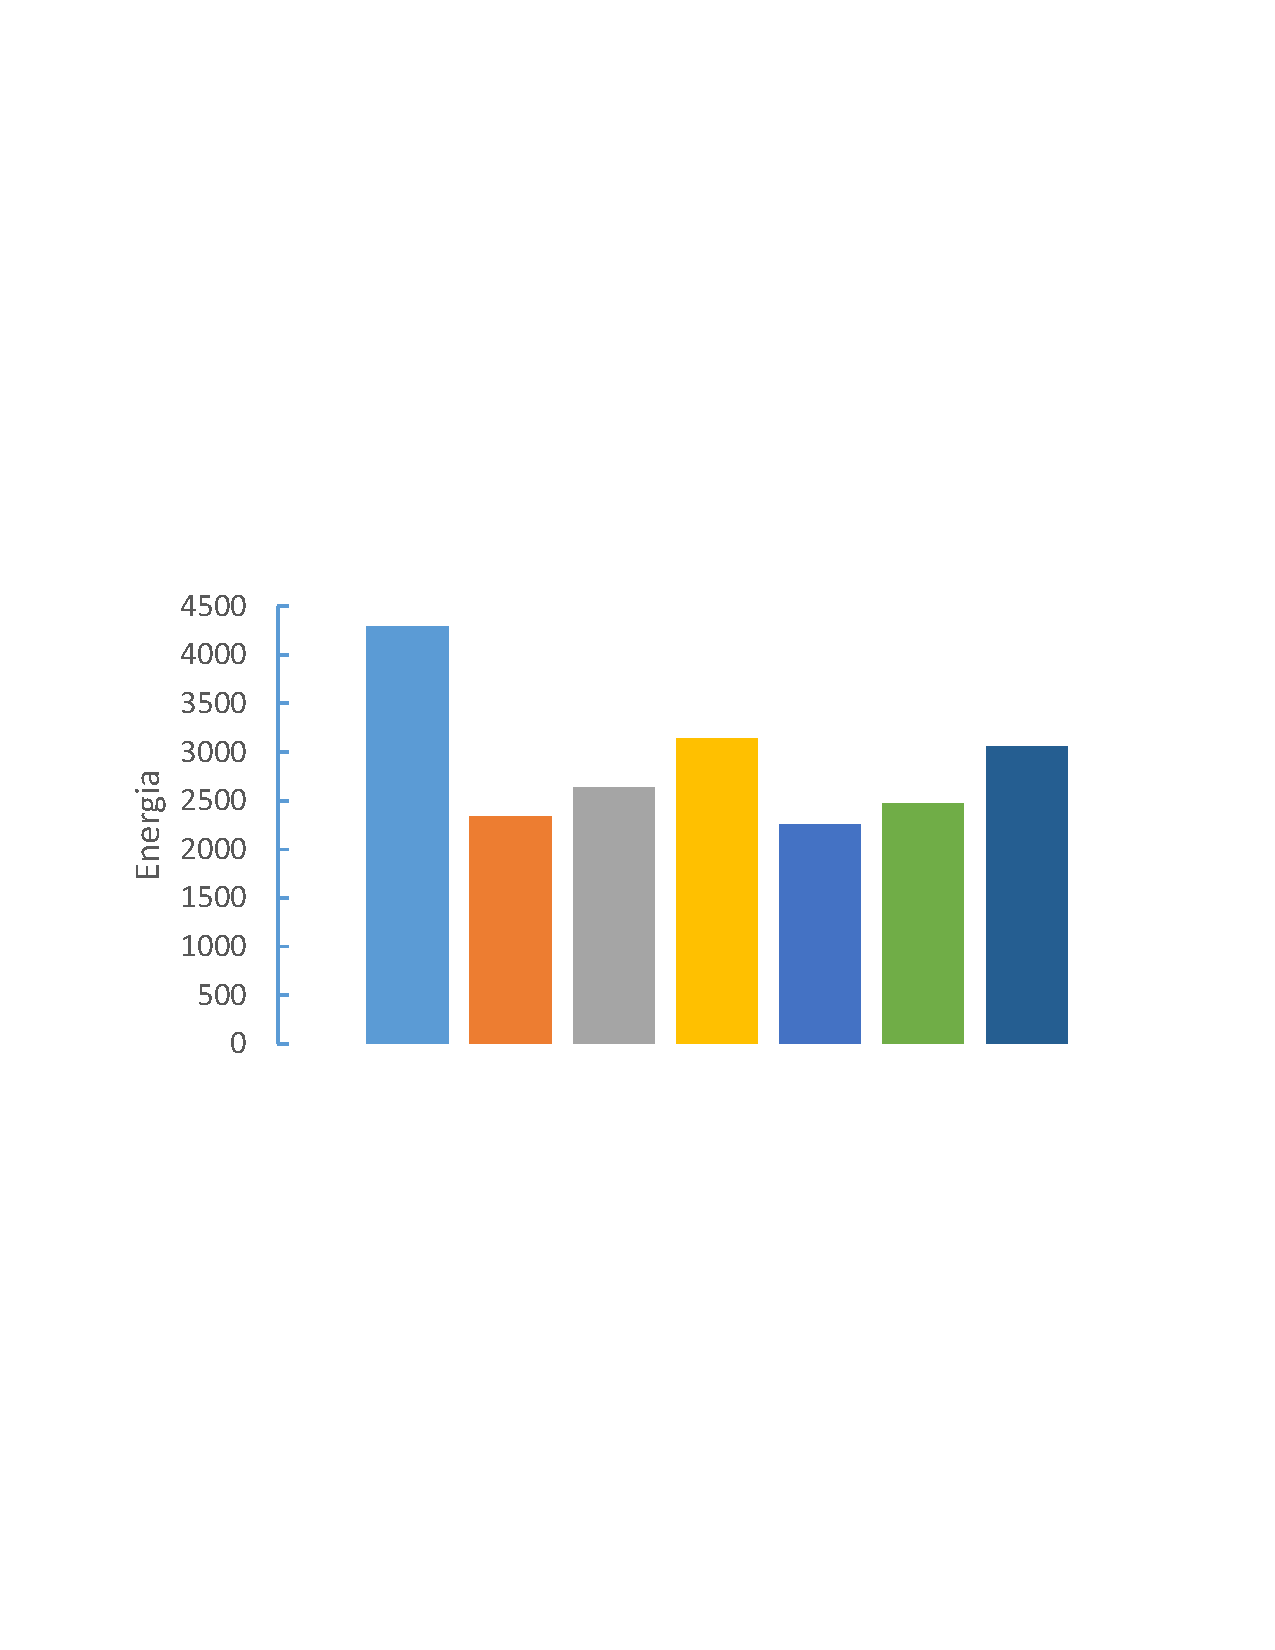
\includegraphics[width= 5cm]{charts/energia_asc.pdf}}\
%\qquad
\subfloat[][]{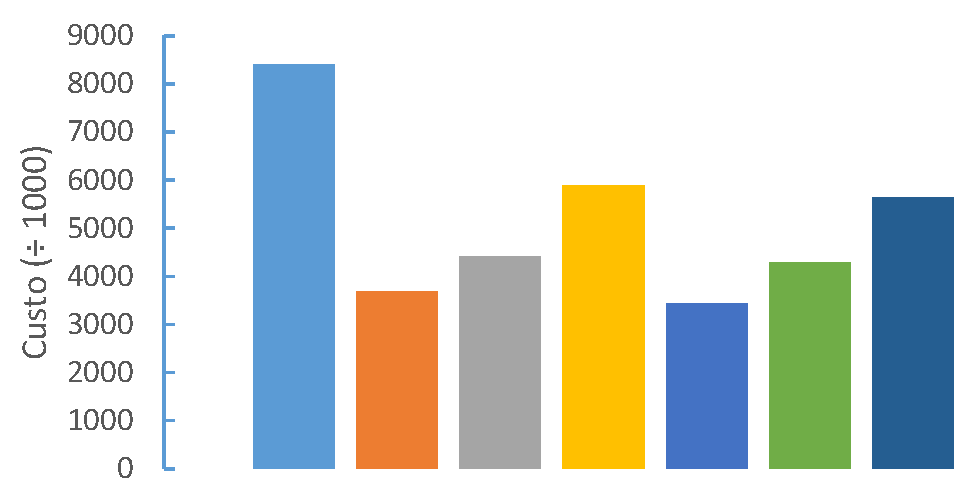
\includegraphics[width= 5cm]{charts/cost_asc.pdf}}\
\caption{Desempenho para aplicação ascendente (cont. R. abrevia para contêineres rígidos e cont. F. para contêineres flexíveis para limite de CPU utilizada)}%
\label{fig:perf_asc}%
\end{figure}
\begin{figure}%
\ContinuedFloat
\centering
\vspace{-0.5\baselineskip}
\subfloat[][]{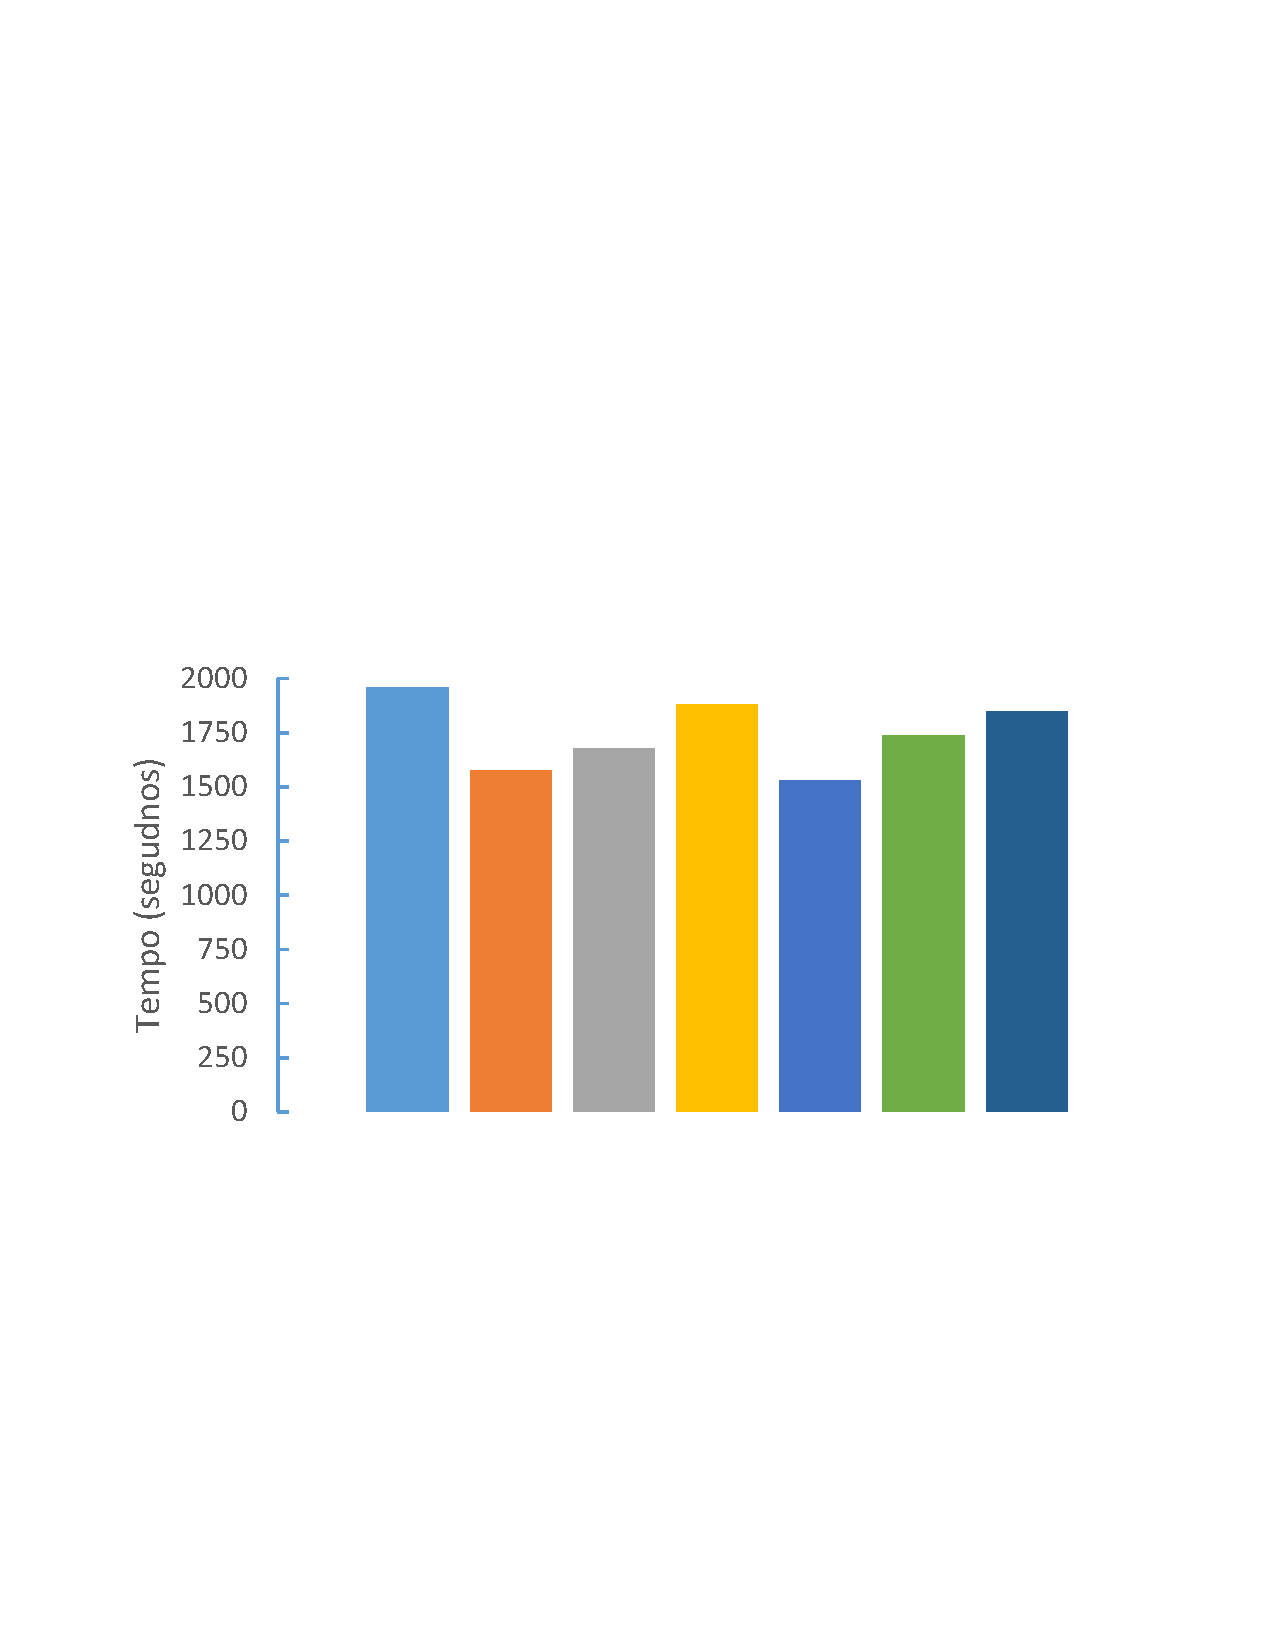
\includegraphics[width= 5cm]{charts/tempo_asc.pdf}}\
%\qquad
\subfloat[][]{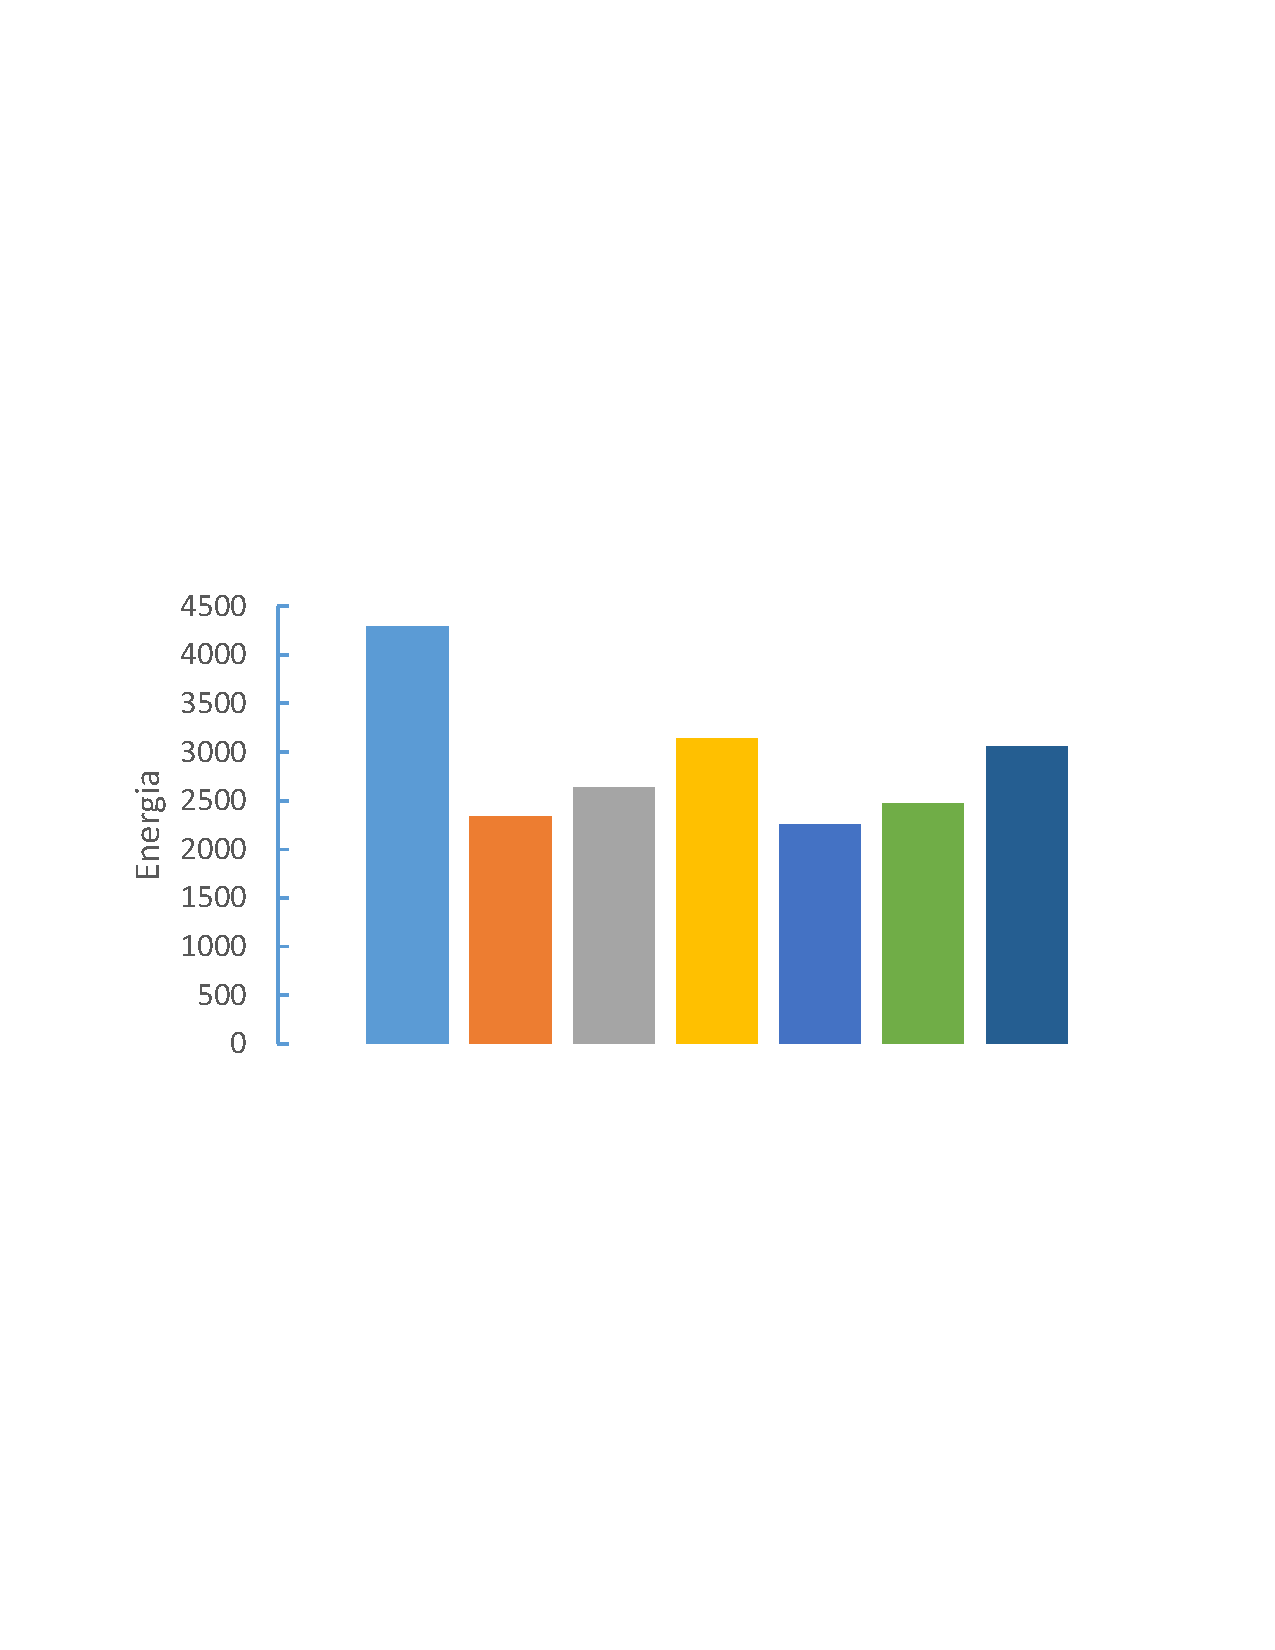
\includegraphics[width= 5cm]{charts/energia_asc.pdf}}\
%\qquad
\subfloat[][]{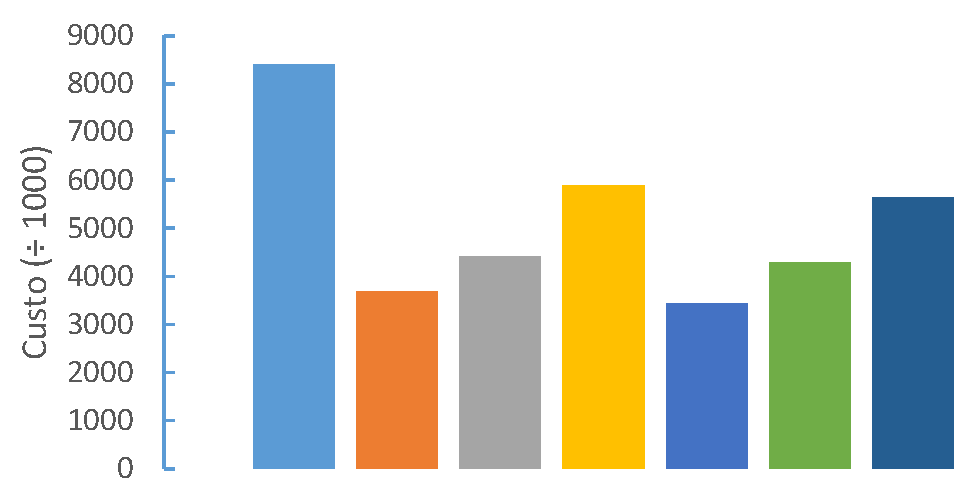
\includegraphics[width= 5cm]{charts/cost_asc.pdf}}\
\caption{Desempenho para aplicação descendente (cont. R. abrevia para contêineres rígidos e cont. F. para contêineres flexíveis para limite de CPU utilizada)}%
\label{fig:perf_des}%
\end{figure}


Colocar um gráfico ilustrando diferença

Comparar especificamente 2 por 2 , fazer uma tabelinha:
Perfil de carga | Virtualização | tempo de alocação | tempo de desalocação | Tempo | Custo
ascending            VM              160                  nao                 


%=======================================================================
% CONCLUSÃO
%=======================================================================
\section{Conclusão}
\label{conclusion}

Descrever aqui o que foi apresentado ``Neste trabalho foi apresentado''. O que houve de contribuição científica.
Diferencial em relação aos trabalhos apresentados. Porque é bom para o mundo.
Possível uso em outras áreas.

- Dados numéricos, números, percentual mais significativo.

%\section{Contribuições Esperadas}
A questão de pesquisa original tratava da possibilidade de se otimizar a camada de virtualização de ambientes em nuvem para execução de aplicações HPC, com o objetivo de identificar também as vantagens e situações onde a virtualização por contêineres pode ser uma melhor alternativa. A partir da avaliação dos trabalhos relacionados, foi concluído que em uma comparação 1 pra 1 de máquina virtual e container, a segunda tecnologia se sobressai em questões de desempenho, confirmando, assim, que é possível otimizar o modelo de elasticidade em nuvem ao substituir a camada de virtualização, passando a utilizar contêineres. Sendo assim, decidimos expandir a questão para analisar o desempenho em situações de elasticidade, onde os recursos precisam ser provisionados conforme a demanda, passando a identificar também o que ocorre e o tempo necessário para as etapas de provisionamento. 

Esperamos também que o modelo e resultados da pesquisa possam servir com um guia para outros pesquisadores poderem identificar qual a tecnologia mais adequada para seus objetivos, a partir da verificação de quais parâmetros são necessários. Pois pretendemos identificar, por exemplo, qual solução é mais indicada para aplicações altamente paralelizadas e cenários onde a variação de consumo de recursos pode variar bastante.

Explicar aqui o que pode ter de furo na implementação, o que não deu tempo de fazer etc.

%=======================================================================
% Referências
%=======================================================================
\bibliography{exemplo}

%=======================================================================
% Exemplo de Apêndice
% O Apêndice é utilizado para apresentar material complementar elaborado
% pelo próprio autor.  Deve seguir as mesmas regras de formatação do
% corpo principal do documento.
%=======================================================================
%\appendix

%=======================================================================
% Exemplo de Anexo
% O Anexo é utilizado para a ``inclusão de materiais não elaborados pelo
% próprio autor, como cópias de artigos, manuais, folders, balancetes, etc.
% e não precisam estar em conformidade com o modelo''.
%=======================================================================
%\annex

\end{document}
